\chapter{Estudo de caso}
\label{cap_estudo_caso}

\section{Introdução}

Realizaremos um estudo de caso múltiplo para avaliarmos o nosso modelo concreto de estimação dos juros da dívida técnica em projetos de software livre descrito no Capítulo \ref{estimacao:juros}.  Com esse estudo de caso, observaremos a adequação do modelo para a avaliação dos juros em projetos reais hospedados em uma plataforma pública de versionamento de software. Adicionalmente, descreveremos a ferramenta GitResearch. Essa ferramenta foi criada para automatizar partes das atividades realizadas durante o estudo de caso.

\section{O repositório de software}

No contexto do \textit{open source}, tornar público o código-fonte de um projeto de software não se trata apenas de uma característica positiva; Na verdade, isso é uma necessidade que caracteriza os princípios dessa filosofia de desenvolvimento de software. A comunidade interessada no software deve ter livre acesso a ele para que possa usá-lo, alterá-lo e distribuí-lo. Por conta dessas necessidades, houve uma popularização dos repositórios públicos de software. Esse tipo de plataforma fornece aos usuários meios para acessar o código  de terceiros como também permite que eles mesmos disponibilizem seus projetos de software. A popularização dessas plataformas fez com que elas fossem a fonte de uma grande quantidade de dados. Esses dados são produzidos de diversas formas. Seja pela extração a partir do código-fonte como também pela interação realizada entre os usuários.  Em todos os casos, a facilidade de acesso e a pluralidade de dados faz com que os repositórios de software sejam uma opção interessante para a obtenção de dados para pesquisas. Em nosso estudo de caso, obteremos dados do GitHub: Um repositório de projetos  de software baseado na tecnologia versionamento Git.



\subsection{Controle de versões utilizando o Git }


Um sistema de controle de versões - ou configurações - é um sistema que fornece uma série de funcionalidades para controlar a evolução de um conjunto de arquivos. Entre essas funcionalidades está ter acesso às versões anteriores de arquivos, controlar quem realizou uma determinada alteração e comparar versões com o intuito de analisar as diferenças.  Além disso, conforme Otte. \cite{otte2009version}, esses sistemas têm sido utilizados como uma ferramenta de backup, pois  permitem voltar a uma versão anterior caso algo esteja errado com a versão atual. O Git é um sistema moderno de controle de versão desenvolvido pelo também criador do Linux Linus Torvalds. Conforme Loeliger et al.\cite{loeliger2012version}, ele pode ser visto como uma evolução de sistemas mais antigos como o CVS\cite{vesperman2006essential} e o Subversion\cite{pilato2008version}. 

O principal diferencial do Git em relação aos outros sistemas de versionamento é a sua característica distribuída. O Git foi projetado para funcionar muito bem em contextos onde exista uma grande quantidade de pessoas interagindo com o mesmo projeto e, ainda assim, haja a necessidade que essa interação ocorra de uma forma organizada e rastreável. Essa característica distribuída é alcançada por meio de alguns recursos:

\begin{itemize}
\item \textbf{Facilidade para a realização de cópias de um repositório}. Qualquer pessoa no mundo pode realizar uma cópia local de um repositório de arquivos público gerenciado por uma instância do sistema Git. Para isso, basta instalar uma versão do Git no computador local e utilizar o comando \textit{clone} seguido pela URL do repositório. \textbf{A cópia obtida contém todo o histórico do projeto como também todos os arquivos necessários para que o versionamento possa ser realizado}. Isso faz com que não exista obrigatoriamente um único repositório central de um determinado projeto. Cada cópia é um repositório independente. 

\item \textbf{É extremamente eficiente comparado às alternativas anteriores.} Uma das razões para essa eficiência está na estratégia utilizado para realizar o controle das versões dos arquivos. No Git existe uma pasta chamada \textit{.git} na pasta onde estão os arquivos sendo gerenciados. Essa pasta contém todos os dados referentes ao histórico dos arquivos como também todas as informações necessárias para realizar o controle de versão. Dessa forma, o Git não precisa acessar a rede para buscar alguma informação necessária para o controle de versão. Todos os dados estão no próprio sistema de arquivos usado para armazenar os arquivos gerenciados. Outra razão da eficiência do Git é a inexistência de um processo que necessariamente precisa estar em execução para que o controle de versão funcione. Isso era necessário nos sistemas anteriores como é o caso do Subversion. Nele havia um \textit{daemon} responsável por realizar o versionamento de arquivos. No Git isso não ocorre. Ao invés disso, o Git fornece um conjunto de programas que ao serem executados conseguem realizar as alterações necessárias nos arquivos de controle de versionamento. 

\end{itemize}


O funcionamento do Git é baseado em um grafo onde cada nó  representa uma versão dos arquivos. Um exemplo dessa organização pode ser visto na Figura \ref{fig:cap_experimento_exemplo_grafo_git}. Nela, um repositório foi iniciado pelo \textit{commit} $C1$ e depois houve uma alteração por meio do \textit{commit} $C2$. Nesse ponto, foram criadas duas novas \textit{branches}. Uma \textit{branch} é um fluxo independente de versões. Normalmente, a \textit{branch} principal de um repositório Git é chamada de master. No exemplo apresentado, os \textit{commit}  $C4$ e $C6$ foram criados a partir do commit $C2$ da \textit{branch} principal. Porém, tanto eles quanto o \textit{commit} $C3$ são totalmente independentes e podem apresentar conteúdos diferentes. Ainda assim, essas linhas independentes de evolução, podem novamente serem combinadas por meio do que é chamado de \textit{merge}. Na Figura \ref{fig:cap_experimento_exemplo_grafo_git_merge}  temos o resultado do \textit{merge} realizado entre as \textit{branches} master e a \textit{branch} 1. A versão obtida após o commit $C8$ contém tanto as alterações que foram realizadas nos \textit{commits} $C4$ e $C5$ quanto as alterações realizadas no commit $C3$. Entretanto, essa operação não traz nenhum impacto à \textit{branch 2}. A criação de \textit{commits}, \textit{branches}, \textit{merges} e todas as outras ações necessárias para o versionamento dos arquivos em um repositório Git são realizado por meio de comandos que esse sistema disponibiliza. Para extrairmos as informações dos projetos analisados nesta pesquisa, utilizaremos alguns desses comandos.  Na Tabela \ref{table:comandos_git} há uma lista com os principais deles e quais as suas funções.  

 \begin{figure}[H]
  \centering
  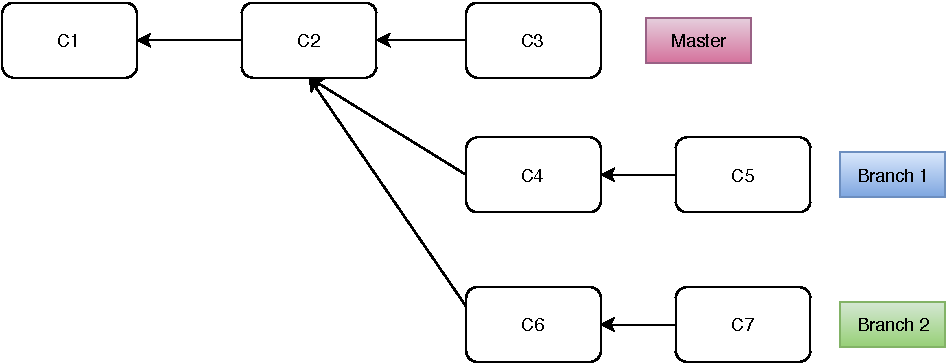
\includegraphics{capitulo_estudo_caso/exemplo_grafo_git.pdf} 
  \caption{Exemplo da estrutura de armazenamento de versões do Git.}
  \label{fig:cap_experimento_exemplo_grafo_git} 
\end{figure}

 \begin{figure}[H]
  \centering
  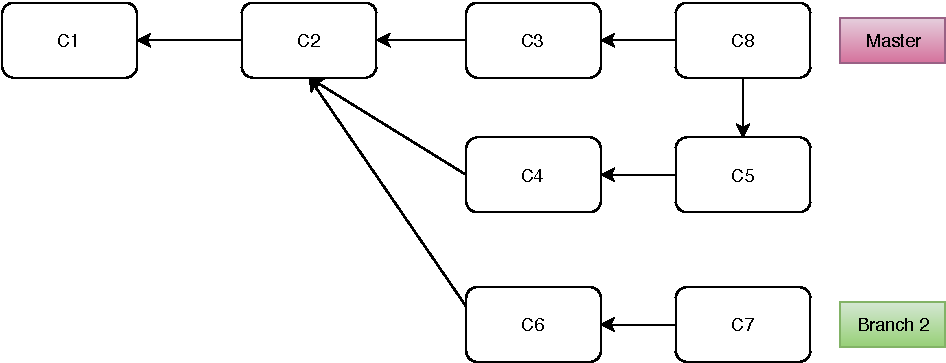
\includegraphics{capitulo_estudo_caso/exemplo_grafo_git_merge.pdf} 
  \caption{Exemplo de merge entre duas \textit{branches}.}
  \label{fig:cap_experimento_exemplo_grafo_git_merge} 
\end{figure}


\begin{table}[H]
\label{table:comandos_git}
\centering
\def\arraystretch{2.5}%
\begin{tabular}{|c|c|c|}
\hline
Comando & \pbox{6cm}{Descrição}                                                     & Exemplo                                     \\ \hline
clone   & \pbox{6cm}{Realiza uma cópia local de um repositório remoto }             & clone https://github.com/torvalds/linux.git \\ \hline
add     & \pbox{6cm}{Inclui um ou mais arquivos no gerenciamento de versão}         & add file.txt                                \\ \hline
commit  &\pbox{6cm} {Efetiva no histórico as mudanças realizadas}                   & commit -m ``History message"                 \\ \hline
push    & \pbox{6cm}{Envia as alterações locais para um repositório remoto}         & git push -u origin branch                   \\ \hline
pull    & \pbox{6cm}{Atualiza os arquivos locais com base em um repositório remoto} & git pull                                    \\ \hline
merge    & \pbox{6cm}{Realiza o merge entre duas \textit{branches}} & merge branch1                                 \\ \hline
branch    & \pbox{6cm}{Cria uma nova branch} & branch branch3                                 \\ \hline
checkout    & \pbox{6cm}{Muda o diretório de trabalho atual para uma determinada branch} & checkout branch3                                 \\ \hline
\end{tabular}
\caption{Comandos básicos do GIT.}
\label{table:comandos_git}
\end{table}


\subsection{GitHub}
\label{cap_estudo_github}

O GitHub é uma plataforma online para o armazenamento de repositórios Git. O que diferencia o GitHub de um servidor Git convencional é o conjunto de funcionalidades adicionais que a plataforma disponibiliza aos seus usuários. Essas funcionalidades são adições aos recursos de versionamento que o Git já disponibiliza como também recursos sociais que permitem a interação entre os usuários. De acordo com  Dabbish et al. \cite{dabbish2012social} essas funcionalidades socias facilitam a colaboração entre os usuários pois viabilizam que eles monitorem as atividades de uma grande quantidade de projetos além de gerar uma grande quantidade de dados. Esses dados, publicamente disponíveis,  tem sido usados ativamente como uma fonte de dados para pesquisas científicas. Entretanto, algumas particularidades dessa plataforma precisam ser devidamente consideradas  para que elas não prejudiquem os resultados dessas pesquisas. Na literatura podemos encontrar algumas recomendações práticas de como evitar problemas na utilização de dados do GitHub em pesquisas científicas \cite{kalliamvakou2014promises,bird2009promises,tsay2014influence}.  Algumas das recomendações que foram consideradas nesta pesquisa durante a fase de extração de dados do GitHub são:

\begin{itemize}
\item \textbf{Nem sempre um repositório no GitHub é utilizado para armazenar um projeto de software.} Apesar de ser voltado para a hospedagem de projetos de software, o GitHub não impõe nenhum tipo de restrição ao conteúdo dos repositórios que ele armazena. Por ser uma plataforma gratuita, isso faz com que muitos usuários o utilizem para o armazenamento de arquivos diversos. Para evitar a inclusão de repositórios que não armazenam projetos de software, utilizamos uma série de heurísticas. Algumas delas sugeridas por Killiamvakou et al.\cite{kalliamvakou2014promises} e outras criadas especificamente para esta pesquisa. 
\item \textbf{Muitos projetos não são totalmente desenvolvidos no GitHub.} Esses desenvolvimento fora do GitHub pode ser de duas formas: prévio e paralelo. Um projeto pode ser desenvolvido previamente em uma outra plataforma e depois ser migrado para o GitHub. Essa migração pode ser feita importando todo o histórico do projeto como também, esse histórico pode ser ignorado. Isso precisa ser considerado já que nesses casos esse histórico anterior pode ser relevante para a pesquisa sendo realizada.  A outra forma de desenvolvimento fora do GitHub é quando algumas das atividades necessárias para o desenvolvimento do projeto não são realizadas no GitHub ou são realizadas parcialmente. Um exemplo seria o gerenciamento de \textit{issues} que pode ser feito no GitHub ou em outro serviço como o FindBugs\cite{ayewah2007using}. Assim, uma pesquisa poderia, equivocadamente, realizar conclusões com base em dados incompletos. O caso em que poderia haver algum impacto nos resultados desta pesquisa é o de desenvolvimento prévio. Caso um projeto fosse criado no GitHub sem que o histórico fosse importando, nossas análises de produtividade não poderiam ser feitas utilizando essa contribuição prévia. Para evitar esse problema, utilizamos, novamente, um conjunto de heurísticas baseadas nas datas de criação dos arquivos do repositório e nas datas dos primeiros \textit{commits} realizados no GitHub. Se um repositório possuía um arquivo com uma data muito anterior ao primeiro \textit{commit}, esse repositório provavelmente teve um desenvolvimento prévio fora do GitHub e, portanto, deveria ser excluído da pesquisa.
\end{itemize}



\subsection{GHTorrent}

O GitHub disponibiliza seus dados por meio de uma API. Nessa API é possível pesquisar informações a respeito de um repositório específico como também buscar repositórios utilizando critérios como linguagem, data de criação e descrição. Porém, devido a questões de segurança, essa API impõe severas restrições de acesso aos seus usuários.  Existe uma quantidade pequena de requisições que podem ser realizadas por hora. Além disso, é necessário um esforço de desenvolvimento para que os dados obtidos possam ser armazenados e principalmente relacionados entre si. Devido a essas dificuldades, surgiram projetos como o GHTorrent, um banco de dados que espelha as informações contidas no GitHub. Esse projeto foi criado por Gousious et al. \cite{gousios2012ghtorrent} para distribuir de uma forma simples e rápida as informações disponibilizadas pela API do GitHub. Ou seja, pesquisadores podem utilizar os dados no GitHub sem ter de desenvolver um sistema que faça a extração desses dados. 

O GHtorrent disponibiliza os dados por meio de arquivos de backup do banco de dados MySql, Big Tables do Google e por meio de um banco de dados online onde os usuários podem se cadastrar e realizar consultas. Escolhemos obter os dados por meio do download de um arquivo de backup do MySql. Optamos por essa forma de acesso, pois queremos incluir uma grande quantidade de projetos em nosso estudo de caso. Por isso, teremos a necessidade de realizar a extração de dados com rapidez. Ao utilizar um backup completo do GHTorrent pudemos importá-lo em um ambiente no qual o poder de processamento fosse compatível com essas nossas expectativas de velocidade.  O arquivo obtido foi o \textit{mysql-2017-12-01}. Esse arquivo contém os dados obtidos até o último dia de dezembro de 2017. A Figura \ref{fig:tabelas_ghtorrent} contém uma lista com as  principais tabelas encontrados no arquivo do GHTorrent e que foram utilizadas nesta pesquisa.


 \begin{figure}[H]
  \centering
  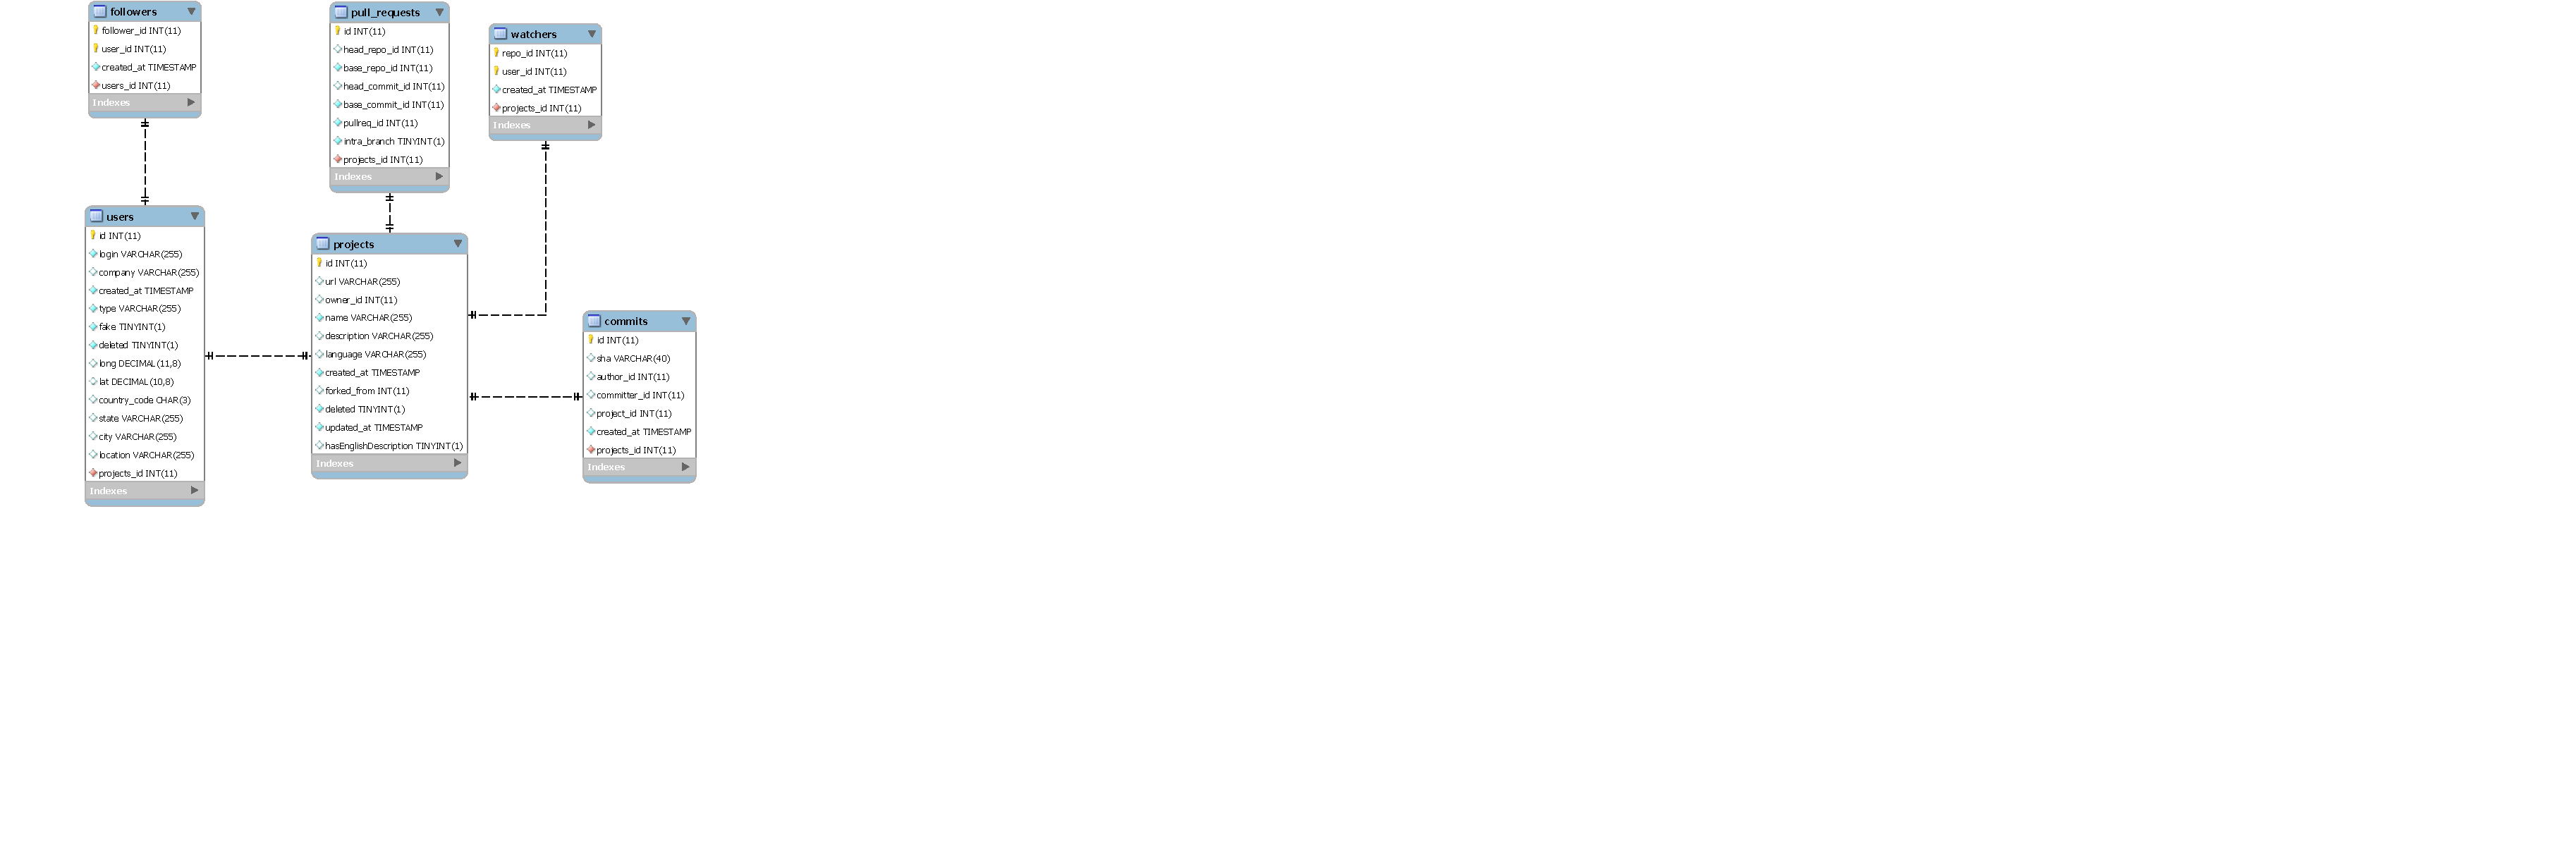
\includegraphics[trim={1cm 7cm 0 0},clip]{capitulo_estudo_caso/tabelas_ghtorrent.pdf} 
  \caption{Tabelas do GHTorrent.}
  \label{fig:tabelas_ghtorrent} 
\end{figure}





\section{Ferramenta de apoio: GitResearch}
\label{cap_estudo_caso_ferramenta}

Construímos uma ferramenta chamada GitResearch para automatizar uma parte das atividades realizadas neste estudo de caso. Essa ferramenta foi desenvolvida na linguagem Java e está disponível em https://github.com/Jandisson/git-research. Uma das razões para a construção dessa ferramenta é a de que ela permitirá que os resultados obtidos nesta pesquisa possam ser reproduzidos.  Além disso, apesar de ter sido desenvolvida especificamente para esta pesquisa, ela foi planejada de forma que possa ser utilizada, com as devidas alterações, em outras pesquisas que envolvam a extração e o  processamento de dados de repositórios de software como o GitHub. Durante a concepção dessa ferramenta, um dos requisitos almejados foi a possibilidade de processar uma grande quantidade de dados utilizando de forma satisfatória o hardware disponível. Isso foi alcançado ao realizar esse processamento de uma forma paralela. Ou seja, a ferramenta foi planejada de forma que as atividades em cada etapa da pesquisa pudessem ser realizadas em diversas linhas de execução. Além disso, houve a preocupação em criar uma arquitetura flexível que facilitasse a alteração das funcionalidades existentes e adição de novas funcionalidades. Para alcançar todos esses objetivos, escolhemos, como a base para o GitResearch, o framework Spring Batch\cite{cogoluegnes2011spring}. Utilizando esse framework vamos executar a tarefa de extração e processamento dos dados como um processo batch. De acordo com Martin. et al. \cite{martin2015batch}, um processamento batch acontece quando casos semelhantes são processados simultaneamente sem a intervenção de um usuário. Escolhemos esse modelo de processamento pois ele se adequa as nossas necessidades de desempenho e condiz com as tarefas que serão realizadas no estudo de caso.



\subsection{Arquitetura}

O GitResearch é baseado na arquitetura do Spring Batch. Um resumo dessa arquitetura é apresentado na Figura \ref{fig:arquitetura_gitresearch}. Um \textit{Job} representa um processo batch. Cada \textit{Job} possui um conjunto, que pode ser ou não ordenado, de \textit{Steps} que por sua vez são as atividades que devem ser realizadas durante o processamento. Tanto um \textit{Job} quanto um \textit{Step} utilizam um repositório de dados chamado de \textit{JobRepository}. Esse repositório armazena, principalmente, dados de controle a respeito de cada execução de um  \textit{Job}. Além disso, o repositório pode ser usado pelos \textit{Steps} para armazenar quaisquer informações que sejam necessárias para realizar o processamento. Cada \textit{Step} é formado por três objetos: \textit{ItemReader}, \textit{ItemProcessor}, \textit{ItemWriter}. Esses três objetos são responsáveis respectivamente por ler, processar e armazenar cada item do processo batch. Cada item será um dos projetos a serem processados neste estudo de caso. 


 \begin{figure}[H]
  \centering
  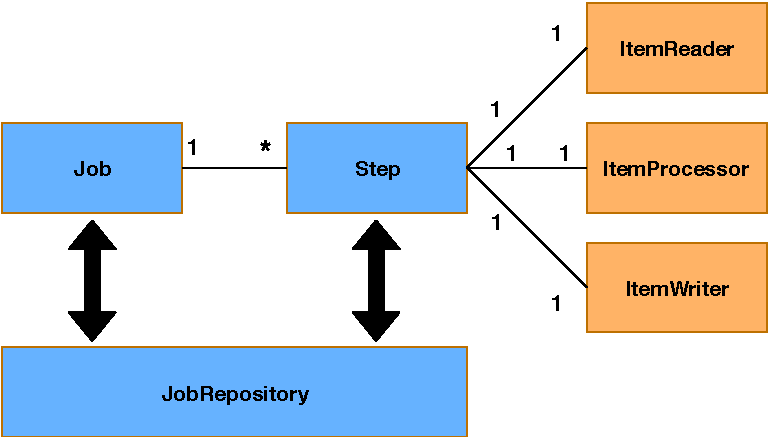
\includegraphics{capitulo_estudo_caso/springbatch_architecture.pdf} 
  \caption{Arquitetura do framework Spring Batch. Adaptada de \cite{minella2011pro}.}
  \label{fig:arquitetura_gitresearch} 
\end{figure}

Os passos realizados para criar o GitResearch, tendo como base o SpringBatch, foram os seguintes:


\begin{enumerate}
\item \textbf{Configuração do JobRepository}. Pode ser usado qualquer banco de dados que tenha suporte ao JDBC\cite{reese2000database}. Em nosso estudo de caso, utilizamos um banco de dados de código livre chamado Derby\cite{mei2010research}.  Ele foi escolhido por ser de fácil configuração e não precisar ser instalado. O banco de dados e gerenciador do banco de dados são armazenados em um único arquivo. Isso facilitará a reprodução do estudo de caso e, consequentemente, a validação dos resultados obtidos.
\item \textbf{Criação e configuração do \textit{Job}}. A configuração de um \textit{Job} consiste em indicar quais \textit{Steps} serão executadas e como essa execução deve ser feita. Nesse ponto é possível determinar qual será o fluxo de \textit{Steps}, se haverá ou não paralelismos  e a quantidade de recursos, como linhas de execução, que deverá ser utilizada. A Figura \ref{fig:configuracao_job} apresenta o código de configuração do \textit{Job} no GitResearch. Em nosso caso, foi necessária apenas a configuração de um \textit{Job}.
\item \textbf{Implementação  dos  \textit{Steps} necessários}. Essa implementação consiste na criação dos \textit{ItemReader}, \textit{ItemProcessor} e \textit{ItemWriter}. Para um determinado \textit{Step}, é possível que não seja necessário criar novos \textit{ItemReader} ou \textit{ItemWriter}. Ao invés disso, é possível utilizar algum objeto previamente criado e disponibilizado pelo framework. Foi isso que foi realizado no GitResearch. A maioria dos \textit{Steps} utiliza algum \textit{ItemReader} ou \textit{ItemWriter} padrão do framework. Entretanto, no caso do \textit{ItemProcessor} não há como utilizar um objeto padrão já que esse elemento é o responsável pela lógica de processamento e isso é particular para cada aplicação. Com isso, a implementação dos \textit{Steps} já existentes no GitResearch como a implementação de novos \textit{Steps}, irá sempre exigir a escrita de novos \textit{ItemProcessor}. No GitResearch foi necessária a implementação de oito \textit{Steps} conforme ilustrado na Figura \ref{fig:passos_gitresearch}.  Conforme mostrado na Figura, a entrada para o processamento realizado pelo GitResearch é uma lista com todos os projetos que serão analisados. Ou seja, essa seleção dos projetos é uma atividade que não é realizada pelo GitResearch. Essa etapa será descrita no item \ref{secao_cap_estudo_selecao_projetos}.
\end{enumerate}



 \begin{figure}[H]
  \centering
   \frame{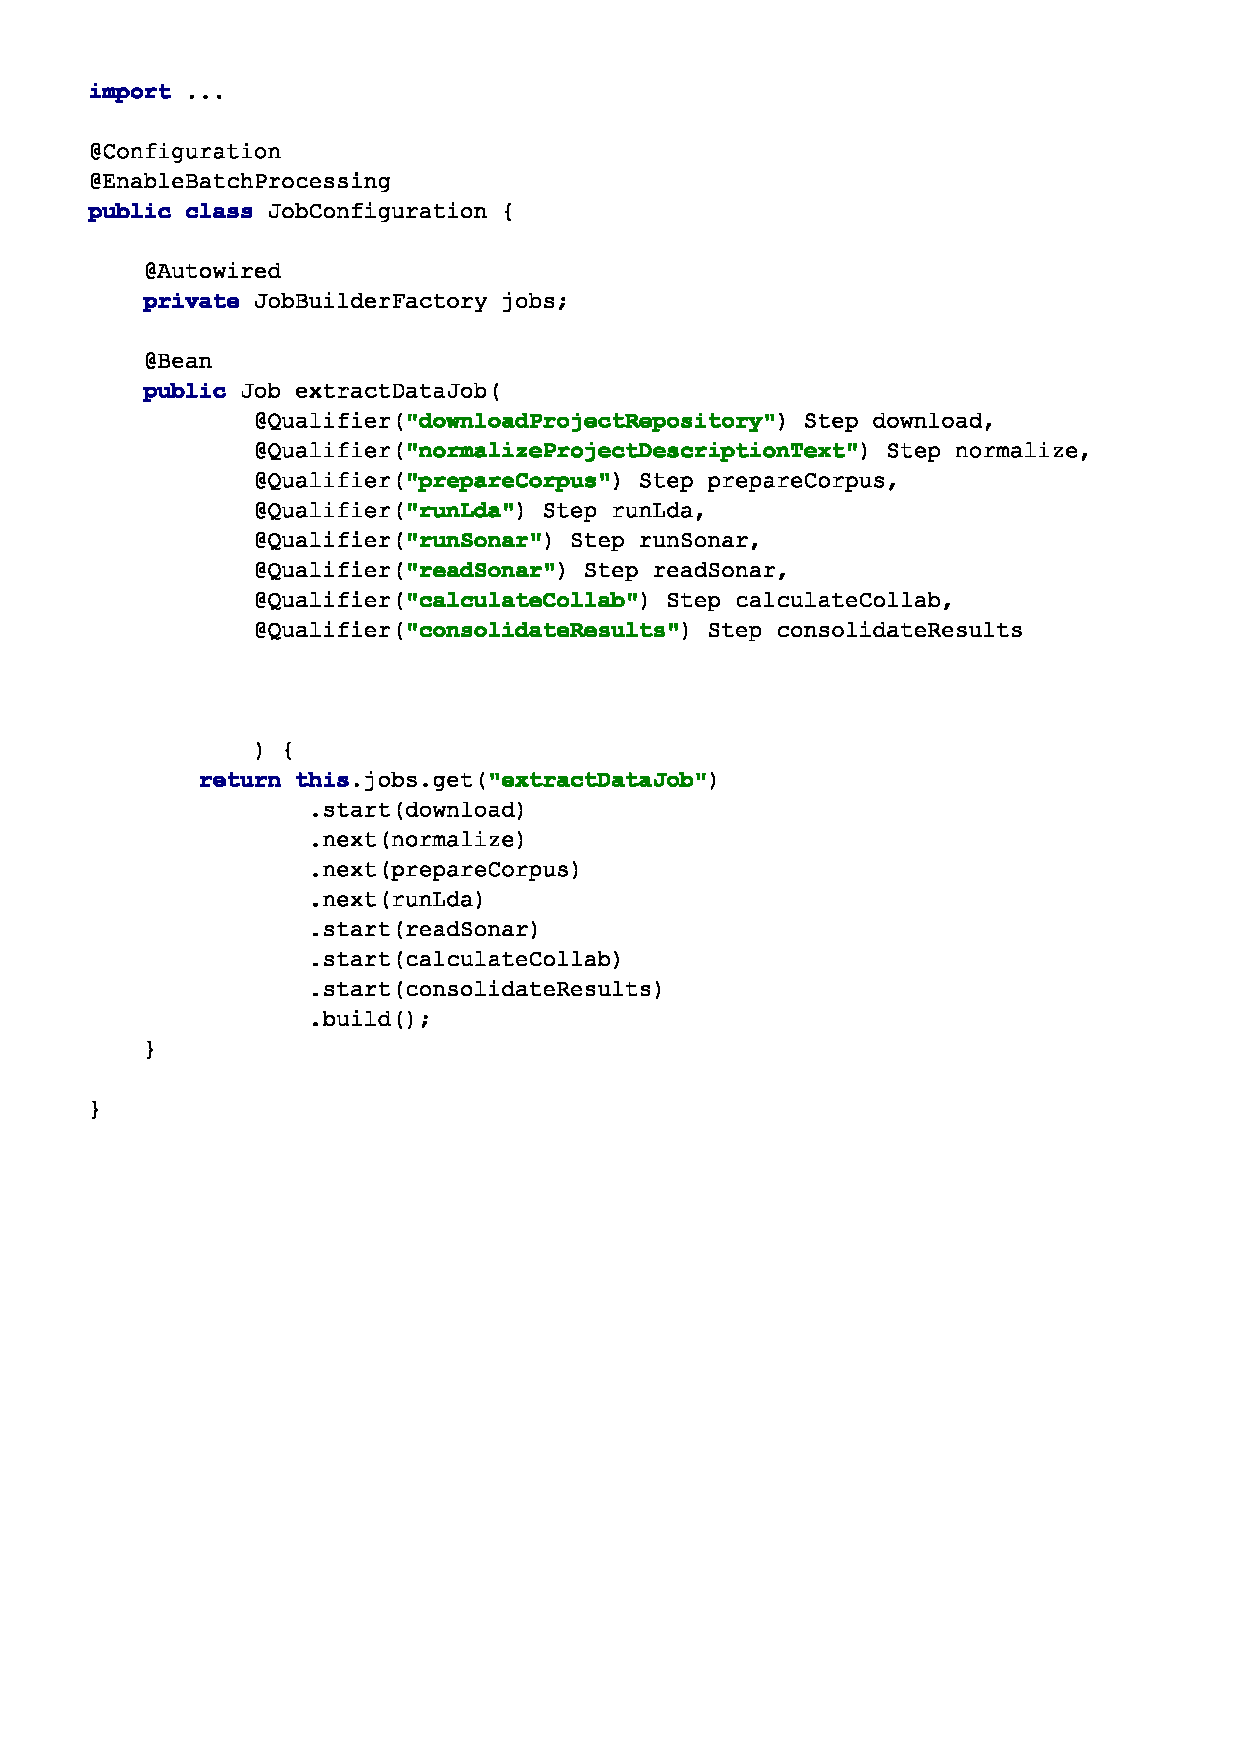
\includegraphics[trim={1cm 10cm 2.5cm 0},clip]{capitulo_estudo_caso/configuracao_job.pdf}} 
  \caption{Código responsável por configurar o \textit{Job} no GitResearch.}
  \label{fig:configuracao_job} 
\end{figure}
 
 


 \begin{figure}[H]
  \centering
  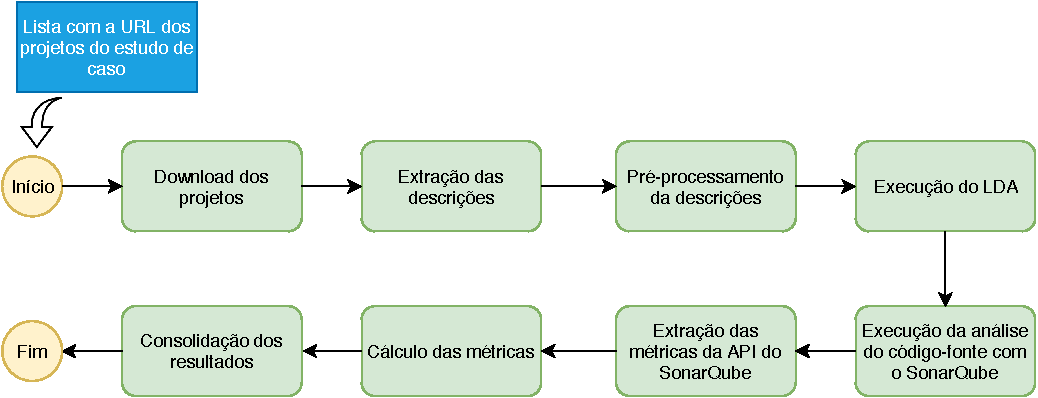
\includegraphics{capitulo_estudo_caso/git_research_steps.pdf} 
  \caption{Passos do processamento no GitResearch.}
  \label{fig:passos_gitresearch} 
\end{figure}



\section{Etapas do estudo de caso}

Nosso estudo de caso foi realizado em seis etapas conforme ilustrado na Figura \ref{fig:cap_metodo_resumo_etapas}. Conforme dito anteriormente, todas essas etapas serão automatizadas ou semiautomatizadas por meio da ferramenta GitResearch. A única exceção é a etapa de seleção dos projetos a serem analisados.  Comparando a Figura \ref{fig:passos_gitresearch} e a Figura \ref{fig:cap_metodo_resumo_etapas}, podemos ver que há diferenças entre as etapas do GitResearch e as etapas do estudo de caso. Isso aconteceu porque algumas etapas do Estudo de caso tiverem de ser divididas no GitResearch em blocos menores. Essa divisão foi realizada tanto por uma questão de coesão quanto de desempenho. Um exemplo é a etapa 2 do estudo de caso. Ela consiste no agrupamento dos projetos que são semelhantes. Esse agrupamento foi realizado aplicando uma técnica de processamento de linguagem natural chamada LDA. Para aplicarmos essa técnica tivemos, antes, que encontrar a descrição do projeto e realizar alguns pré-processamentos. Com isso, a etapa 2 do estudo de caso gerou 3 etapas no GitResearch: extração da descrição, pré-processamento e execução do LDA. Na Figura \ref{fig:cap_metodo_mapeamento_estudo_gitresearch} apresentamos um mapeamento entre as etapas do estudo de caso e as etapas de processamento no GitResearch. A seguir descreveremos a execução de cada uma das etapas do estudo de caso. 






  \begin{figure}[H]
  \centering
  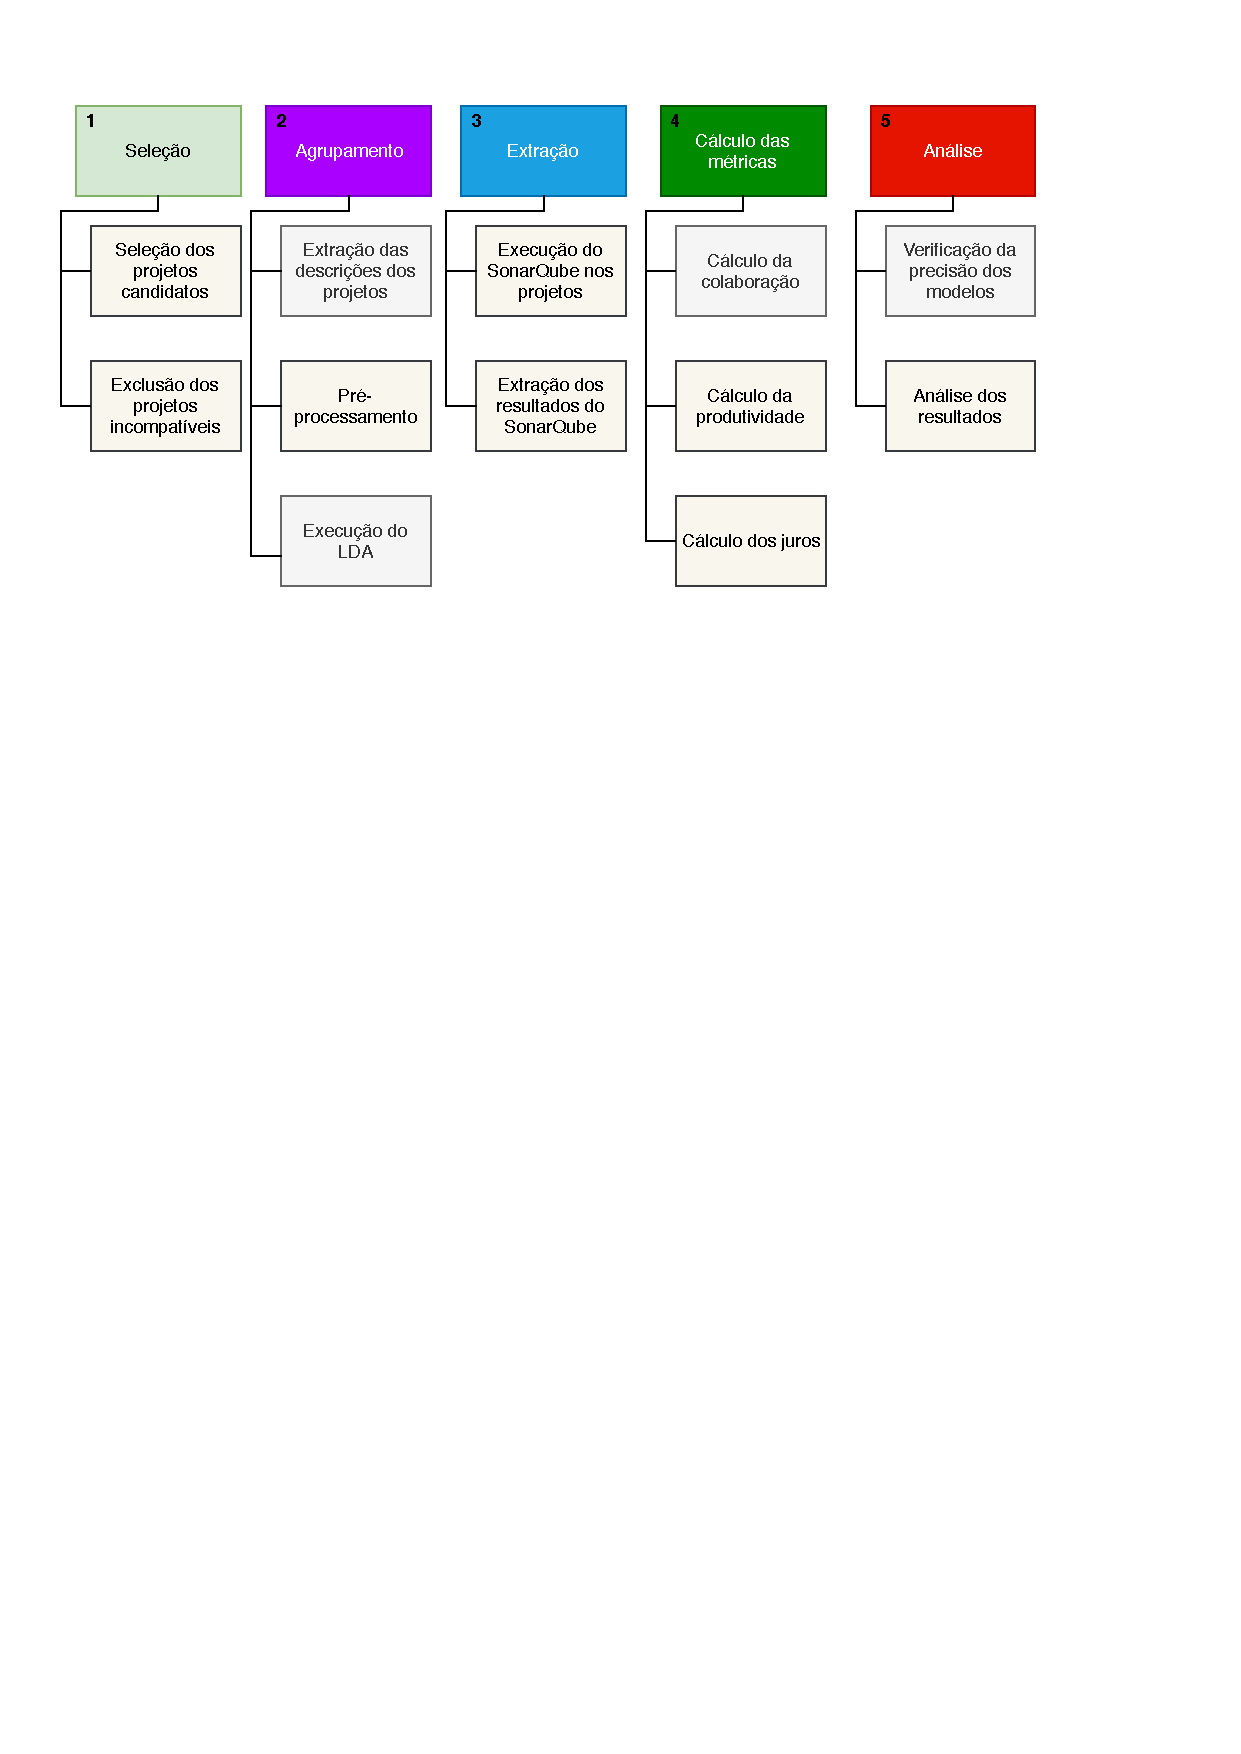
\includegraphics{capitulo_metodo/ResumoEtapas.pdf} 
  \caption{Resumo das etapas do estudo de caso. }
  \label{fig:cap_metodo_resumo_etapas} 
\end{figure}

  \begin{figure}[H]
  \centering
  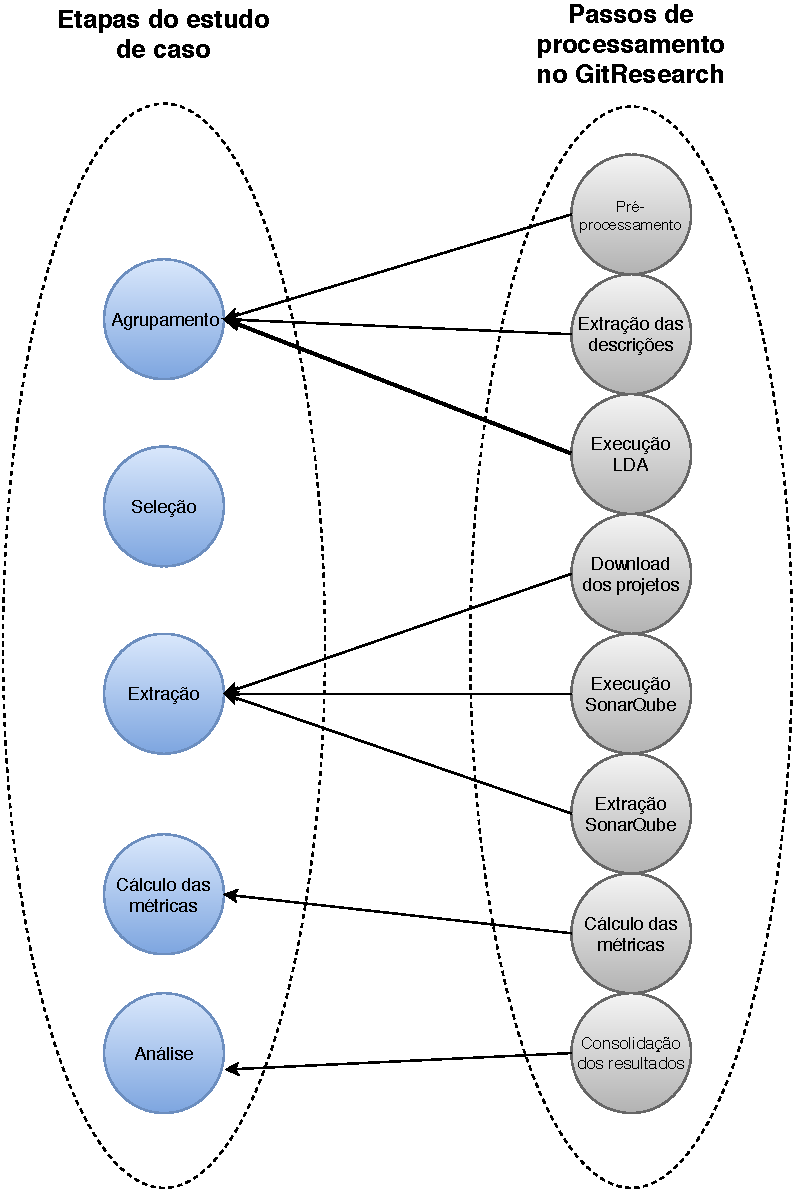
\includegraphics{capitulo_estudo_caso/mapeamento_etapas_estudo_gitresearch.pdf} 
  \caption{Mapeamento entre as etapas do estudo de caso e as etapas de processamento no GitResearch. }
  \label{fig:cap_metodo_mapeamento_estudo_gitresearch} 
\end{figure}


\subsection{Seleção dos projetos}
\label{secao_cap_estudo_selecao_projetos}

A seleção dos projetos a serem incluídos neste estudo de caso foi realizada utilizando um conjunto de regras de exclusão. Ou seja, inicialmente selecionamos todos os projetos armazenados no GitHub e depois essas regras de exclusão foram aplicadas fazendo com que o número de projetos diminuísse. Essa estratégia foi usada porque nosso objetivo era incluir a maior quantidade de projetos possível e com isso diminuir a possibilidade de criação de algum viés caso fossem selecionados projetos específicos. Acreditamos que com isso, a amostra de projetos selecionados é uma representação estatisticamente relevante da população de projetos existentes no GitHub.  As regras de exclusão foram definidas observando três grupos de aspectos da pesquisa:

\begin{enumerate}
\item \textbf{Restrições metodológicas.} Esse grupo de regras inclui aquelas criadas pela necessidade de excluir alguns projetos por eles não possuírem alguma característica que era obrigatória para a aplicação de algum aspecto da metodologia definida para a pesquisa. Um exemplo é a exclusão de projetos no qual a descrição não estava na língua inglesa. Essa regra foi criada porque a análise de projetos em múltiplas línguas não é compatível com a atividade de agrupamento de projetos semelhantes. Para essa atividade utilizamos uma técnica de processamento de linguagem natural chamada LDA. Essa técnica agrupa as descrições dos projetos utilizando como base o número de ocorrência de palavras. Se por exemplo, uma descrição contém diversas vezes as palavras \textit{management} e \textit{database}, o LDA irá criar um tópico com essas duas palavras e inserir nele todos os projetos que possuem também muitas ocorrências dessas duas palavras. Provavelmente, os projetos incluídos serão gerenciadores de banco de dados ou projetos relacionados. Entretanto, caso sejam incluídos projetos de gerenciadores de banco de dados no qual a descrição esteja em outro idioma, e as palavras \textit{management} e \textit{database} fossem escritas nesse idioma, esses projetos poderiam ser colocados em outro tópico. Ou seja, projetos de um mesmo domínio seriam agrupados em grupos diferentes apenas por causa da diferença no idioma da descrição. Por essa razão, foi criada uma regra que removeu todos os projetos que não estavam com a descrição em inglês. Foi escolhido o idioma inglês, pois a aproximadamente 70\% dos projetos no GitHub estavam documentados em inglês.
\item \textbf{Restrições operacionais.} Nesse grupo de regras estão aquelas que foram criadas devido a limitações operacionais durante a realização do estudo de caso. Essas restrições, na maior parte das vezes, foram encontradas nas ferramentas utilizadas em algumas etapas da pesquisa. Um exemplo é a ocorrência de falhas durante  a extração das métricas do código-fonte utilizando a ferramenta SonarQube. Alguns projetos não puderam ter seu código-fonte analisado por essa ferramenta mesmo após diversas tentativas e o acionamento do suporte da ferramenta. Com isso, esses projetos tiveram de ser excluídos já que uma extração manual dessa métricas era inviável devido ao tamanho dos projetos. Ainda nesse grupo de regras de exclusão estão aquelas que foram criadas devido a imcompatibilidade com o sistema operacional utilizado. Alguns arquivos tinham nomes muito extensos ou utilizavam caracteres que não eram aceitos pelo sistema operacional que foi utilizado para a execução do estudo de caso. Isso levou a exclusão dos projetos que continham os arquivos que geraram esses problemas.
\item \textbf{Inclusão apenas de repositórios de software. } O último grupo de regras é formado por aquelas que foram criadas para excluir repositórios que não sejam projetos de desenvolvimento de software. Conforme já dito no item \ref{cap_estudo_github}, muitos dos repositórios criados no GitHub são usados apenas para armazenar arquivos. Para excluir esses repositórios nós utilizamos regras sugeridas pela literatura. Além disso, após a realização de análises preliminares da lista de projetos, também criamos nossas regras de exclusão. Com isso, um número substancial de repositórios foi removido da pesquisa. 
\end{enumerate}

A Tabela \ref{table:regras_exclusao} contém uma lista com todas as regras de exclusão utilizadas para a seleção dos projetos. As regras estão ordenadas na tabela na ordem em que foram aplicadas. Nessa tabela fornecemos uma descrição da regra, indicamos se ela se trata de uma regra metodológica, operacional ou para verificar se o repositório é realmente um projeto de software. Além disso, informamos se a regra foi aplicada utilizando como base os dados no GHTorrent ou houve a necessidade de acessar o código-fonte do projeto.  Por fim, informamos a quantidade de projetos que foram removidos por cada regra de exclusão. 



É necessário detalhar a motivação de algumas das regras de exclusão criadas. Uma delas é a regra número 4 foi criada para evitar que projetos duplicados fossem incluídos na pesquisa. No GitHub, um \textit{Fork} é um procedimento onde um usuário realiza uma cópia, para a sua conta, de um repositório \cite{thung2013network}. Esse procedimento é realizado quando esse usuário deseja contribuir com esse repositório original ou quando ele tem interesse em iniciar um novo projeto tendo como base esse repositório inicial. Em ambos os casos, esses dois repositórios serão muito parecidos. Logo, resolvemos remover esses repositórios que foram gerados por meio de um \textit{Fork}. Outra regra que precisa ser esclarecida é a de número 7. Removemos os projetos que tinham menos de 6 colaboradores e um número de \textit{commits} menor do que 516. Essa exclusão foi realizada com o objetivo de remover da pesquisa os repositórios que não são projetos de software. De acordo com Bird et al.\cite{bird2009promises}, o número de colaboradores e o número de \textit{commits} são uma forma eficaz de identificar repositórios que tenham sido criados apenas para a realização de testes, que sejam exemplos de código ou que sejam projetos particulares. De acordo com os autores,  se um repositório teve uma quantidade mínima de \textit{commits} e colaboradores, há uma probabilidade maior de que seja um projeto de software real. Os números mínimos utilizados nesta pesquisa foram obtidos por meio de análises dos projetos existentes no GitHub. Foi encontrada uma média desses números em todo o conjunto de projetos do GitHub e a essa média foi adicionada uma margem de dois desvios padrão. Por fim, a regra 11 permitiu a exclusão de projetos com uma quantidade muito grande de arquivos para serem analisados. Essa regra foi criada por dois motivos. O primeiro foi a impossibilidade de o SonarQube processar alguns desses projetos. Mesmo após diversas tentativas e o acionamento do suporte da ferramenta, não pudemos processá-los. O segundo motivo é a observação de que repositórios com muitos arquivos normalmente não são projetos de software. Ao invés disso, eles são criados para armazenar logs e outros tipos de arquivos que não tem relação com o desenvolvimento de software.

No banco de dados do GHTorrent há um total de 72.433.097 repositórios. Após a aplicação das onze regras de exclusão listadas na Tabela \ref{table:regras_exclusao}, sobrou um total de 1.867 repositórios.  Ou seja, neste estudo de caso analisaremos 1.867 repositórios de software.





\def\arraystretch{2.5}
\begin{longtable}{|c|c|c|c|c|}

\hline
\# & \pbox{8cm}{Descrição}                                                                            & Tipo     & Local     & \pbox{1.7cm}{Projetos Excluídos} \\ \hline
1  & \pbox{8cm}{Exclusão de projetos abandonados, exemplos, exercícios, tutoriais e projetos android.} & Software & GHTorrent &     20.512.394      \\ \hline
2  & \pbox{8cm}{Exclusão de projetos que não utilizem a linguagem de programação Java.} & Metodológica & GHTorrent &    48.385.193       \\ \hline
3  & \pbox{8cm}{Exclusão de projetos deletados.} & Software & GHTorrent &    367.570       \\ \hline
4  & \pbox{8cm}{Exclusão de projetos que são \textit{Forks} de outros projetos.} & Metodológica & GHTorrent &    1.637.704       \\ \hline
5  & \pbox{8cm}{Exclusão de projetos sem descrição no GHTorrent.} & Metodológica & GHTorrent &     595.557      \\ \hline
6  & \pbox{8cm}{Exclusão de projetos no qual a descrição não esteja em inglês.} & Metodológica & Código-fonte &     342.925      \\ \hline
7  & \pbox{8cm}{Exclusão de projetos que tenham poucos \textit{commits} e poucos colaboradores.} & Software & GHTorrent &    588.909       \\ \hline
8  & \pbox{8cm}{Exclusão de projetos com nomes de arquivos incompatíveis.} & Operacional & Código-fonte &  126         \\ \hline
9  & \pbox{8cm}{Exclusão de projetos no qual o SonarQube não foi capaz de analisar o código.} & Operacional & Código-fonte &      54     \\ \hline
10  & \pbox{8cm}{Exclusão de projetos com arquivo de descrição inexistente ou muito pequeno .} & Metodológica & Código-fonte &   726        \\ \hline
11 & \pbox{8cm}{Exclusão de projetos muito grandes .} & Operacional & Código-fonte &      72     \\ \hline



\caption{Regras para a exclusão de projetos do estudo de caso}
\label{table:regras_exclusao}
\end{longtable}
\def\arraystretch{1}


\section{Agrupamento dos projetos}

Nosso modelo de estimação dos juros da Dívida técnica é baseado na comparação das produtividades de projetos que possuam pouca dívida técnica e projetos que possuem um nível médio ou alto da dívida técnica. Entretanto, essa comparação será feita apenas entre projetos de um mesmo domínio de aplicação. Por exemplo, arcabouços de desenvolvimento como o Spring Batch\cite{cogoluegnes2011spring}, que foi usado para desenvolver a ferramenta GitResearch, só terá sua produtividade comparada com outros projetos que também sejam arcabouços de desenvolvimento ou estejam relacionados a arcabouços de desenvolvimento.  Neste estudo de caso, realizaremos esse agrupamento dos projetos por domínio utilizando uma técnica de processamento de linguagem natural chamada \textit{Latent Dirichlet Allocation}( LDA). Extrairemos de cada projeto a sua descrição e aplicaremos o LDA para identificar o seu domínio.

\subsection{LDA}

O LDA considera que um documento é formado por palavras que por sua vez estão relacionadas a um tópico.  As palavras são associadas a um tópico automaticamente durante a análise do conjunto de documentos. Se uma palavra $w_1$ aparece em muitos documentos junto com uma palavra $w_2$, o LDA assume que há uma relação semântica entre essas palavras e por isso elas devem ficar em um mesmo tópico. Um exemplo seriam as palavras \textit{player}, \textit{game} e \textit{joystick}. Essas palavras normalmente seriam muito encontradas nas descrições dos projetos relacionados aos jogos eletrônicos. Isso faria com o LDA criasse um tópico com essas e outras palavras relacionadas aos jogos e associasse esse tópico a todos os documentos no qual elas aparecem muitas vezes. O LDA baseia-se na ideia de que cada documento analisado foi gerado por uma combinação de  X\% de palavras de um tópico $A$, Y\% de um tópico $B$ e assim por diante. Sendo assim, dado um documento $D$, o LDA realiza o caminho inverso  para identificar o quanto do tópico $A$ foi usado para gerar o documento $D$, o quanto do tópico $B$ foi usado para gerar o documento $D$ e assim por diante.  Em nosso estudo de caso esses documentos serão os textos com a descrição dos projetos. Consideraremos que dois projetos são similares se os tópicos mais presentes em cada um deles são iguais. 


\subsection{A aplicação do LDA}



A primeiro item a ser definido antes da aplicação do LDA em um conjunto de documentos é a definição de quantos tópicos serão utilizados. Neste estudo de caso, utilizamos o número 30. Esse número foi escolhido após a realização de experimentos onde vários números foram testados. Com uma quantidade muito grande de tópicos percebemos que alguns deles ficaram com apenas um ou nenhum projeto. Quando um número muito pequeno de tópicos foi escolhido, percebemos que alguns dos tópicos gerados claramente misturavam mais de um assunto. Além disso, o número 30 foi escolhido por ser um número próximo do utilizados em outros trabalhos semelhantes como o de Ray et al.\cite{ray2014large}. 

Para a execução do LDA foi necessário extrair a descrição de cada projeto. Essa descrição foi obtida do próprio repositório onde o projeto é armazenado. Isso pôde ser feita já que há uma padronização em relação ao nome do arquivo onde a descrição do projeto deve ser inserida. Esse arquivo fica localizado no diretório raiz do repositório e normalmente recebe o nome de \textit{readme.md}. Entretanto, é possível que sejam usadas variações desse nome como \textit{readme.txt} e \textit{readme.html}. Quando nem  o arquivo padrão nem  alguma das variações foi encontrada, foi utilizado qualquer arquivo no qual o nome inicia com a palavra readme. Se mesmo assim, não foi encontrado nenhum arquivo, então o projeto foi excluído da pesquisa conforme a regra 10 da Tabela \ref{table:regras_exclusao}.

Após a extração da descrição de cada projeto, foi necessário realizar uma série de manipulações textuais nas descrições de tal  forma que  elas pudessem ser utilizadas com o LDA. Essas manipulações incluem a remoção de palavras irrelevantes como preposições e artigos, remoção de marcações HTML e XML, a remoção de caracteres especiais e a redução de palavras para sua forma comum(\textit{stemming}\cite{jivani2011comparative}).  Essas modificações foram realizada no GitResearch por meio da classe \textit{DescriptionNormalizer}. Cada uma das transformações foi escrita em uma classe individual e inseridas no grupo padrão de transformações. Em outras pesquisas, será possível criar novos grupos de transformações.  A Tabela \ref{table:transformacoes_lda} apresenta uma lista com todas as classes de transformação que foram utilizadas no pré-processamento das descrições.


\begin{table}[H]

\def\arraystretch{2.5}
\begin{tabular}{|c|c|}

\hline
Classe                                 & \pbox{8cm}{Transformação}                                                                            \\ \hline
RemoveUrlTransformation                & \pbox{8cm}{Remove todas as URL do texto }                                                            \\ \hline
RemoveXmlTransformation                & \pbox{8cm}{Remove todas as marcações HTML e XML}                                                     \\ \hline
RemoveEspecialCharactersTransformation & \pbox{8cm}{Remove caracteres especiais}                                                              \\ \hline
RemoveSpacesTransformation             & \pbox{8cm}{Remove espaços múltiplos}                                                                 \\ \hline
RemoveNumbersTransformation            & \pbox{8cm}{Remove todos os números}                                                                  \\ \hline
LowerCaseTransformation                & \pbox{8cm}{Transforma todo o texto em minúsculo}                                                    \\ \hline
RemoveStopWordsTransformation          & \pbox{8cm}{Remove palavras como "the" e "and" que são irrelevantes  para a categorização dos textos} \\ \hline
RemoveLicenseWordsTransformation       & \pbox{8cm}{Remove texto a respeito das licenças dos softwares}                                      \\ \hline
\end{tabular}
\def\arraystretch{1}
\caption{Transformações realizadas no texto das descrições dos projetos}
\label{table:transformacoes_lda}
\end{table}


\subsection{Resultado do LDA}

A Tabela \ref{table:topicos_lda} apresenta todos os 30 tópicos e suas respectivas palavras. Conforme pode ser visto, as palavras estão em sua forma reduzida devido à aplicação do \textit{stemming}. Um exemplo pode ser visto no Tópico 12. A primeira palavra desse tópico é a palavra ``test''. Entretanto, na verdade, essa palavra representa todas as palavras que contém o prefixo ``test'', como ``testing'', ``tests'', ``testability'' e assim por diante. 

É importante destacar que as palavras estão sendo exibidas na tabela \ref{table:topicos_lda} ordenadas pelo seu nível de relevância dentro do tópico. Por isso, para identificar qual domínio cada tópico representa, a primeira palavra deve ser a mais decisiva.  Existem alguns tópicos no qual as suas palavras permitem-nos claramente identificar o domínio que ele representa. Esse é o caso do tópico 22 que agrupará os projetos relacionados aos jogos eletrônicos. Outro exemplo é o Tópico 23 que agrupará projetos relacionados ao processamento distribuído de dados. Enquanto isso, alguns tópicos não nos permitem identificar qual domínio eles representam. 



\def\arraystretch{2.5}
\begin{longtable}{|c|c|}
\hline
Nome & \pbox{13cm}{ Palavras}                                                                                                                                             \\ \hline
Tópico 1          & \pbox{13cm}{applic android fix xprivacy addon restrict support ad data devic forg app play improv processor return permiss mode googl map }                       \\ \hline
Tópico 2          & \pbox{13cm}{index elasticsearch cassandra data set search json type file query solr field document fs true default test map bin support}                          \\ \hline
Tópico 3          &\pbox{13cm}{ build instal java run file jar directory packag ant sourc command window download compil path test linux document git bin }                           \\ \hline
Tópico 4          &\pbox{13cm}{ connect client server user authent command default host session key configur ssh option password set login request winrm overther file}               \\ \hline
Tópico 5          &\pbox{13cm}{ query api custom item id storefront checkout respons field widget java chart content overrid v1 terasoluna type gfw public payment }                  \\ \hline
Tópico 6          & \pbox{13cm}{distribut export wicket includ govern inform encrypt law file h2o security requir build impli kind cryptograph applic country import condit}          \\ \hline
Tópico 7          &\pbox{13cm}{ docker servic run imag doc user contain cluster api creat meso aw compos configur karaf url command provid build jame}                                \\ \hline
Tópico 8          & \pbox{13cm}{stream sampl data event file configur messag parser log queue tnt4j activ xml defin field property string chronicl paramet entri}                     \\ \hline
Tópico 9          & \pbox{13cm}{applic develop servic manag web support data base system server framework user compon model build platform api integr document modul}                 \\ \hline
Tópico 10         & \pbox{13cm}{java report attribut set job user operationresult resourc servic row session method id column client jasperadmin organ request list server}           \\ \hline
Tópico 11         & \pbox{13cm}{java class method public string type return annot builder final object map static xml gener interfac org api void person}                             \\ \hline
Tópico 12         & \pbox{13cm}{test driver tabl databas java run jdbc engin configur execut gwt sql default requir assert selenium junit user connect firefox}                       \\ \hline
Tópico 13         &\pbox{13cm}{ issu contribut build develop sourc document code statu support list maven download badg open bug request mail doc api wiki}                           \\ \hline
Tópico 14         & \pbox{13cm}{java core imag question demo src main aima text link student answer ui search org jar library post bridgedb afc}                                      \\ \hline
Tópico 15         & \pbox{13cm}{graph java data algorithm handlebar src script templat workflow input comment structur output languag code taverna jwetherel compil task yesworkflow} \\ \hline
Tópico 16         & \pbox{13cm}{file library format imag jar support data gnu gener includ sourc java public code free distribut form common term work}                               \\ \hline
Tópico 17         &\pbox{13cm}{ click sdk select modul file elixir function tab run png screenshot button line true configur menu test open view raw}                                 \\ \hline
Tópico 18         & \pbox{13cm}{matrix de jsf msf4j openbaton implement jersey opengl microservic chouett redisson build matrix4f baton microserv joml transform en dddlib ob1k }     \\ \hline
Tópico 19         & \pbox{13cm}{test simul run remot worker coordin hazelcast start client command agent machin member predict file benchmark cflint java script map}                 \\ \hline
Tópico 20         & \pbox{13cm}{file set code support option creat time number work make note provid class chang type default configur user system includ}                            \\ \hline
Tópico 21         &\pbox{13cm}{ run server databas instal test configur applic file build start deploy properti tomcat mysql user mvn default web db war}                             \\ \hline
Tópico 22         &\pbox{13cm}{ game mod player minecraft team robot openmr block server main make item build play develop creat place piec gener asset}                              \\ \hline
Tópico 23         &\pbox{13cm}{ build eclips plugin run test maven instal mvn gradl jar gradlew repository java file modul command id target clean org}                               \\ \hline
Tópico 24         & \pbox{13cm}{data model research analysi databas tool develop rif univers genom gener base public peptideshak comput health repository inform sourc design}        \\ \hline
Tópico 25         & \pbox{13cm}{data hadoop spark cluster distribut index node oper read random algorithm process scala exampl deep learn model machin comput pipelin}                \\ \hline
Tópico 26         & \pbox{13cm}{api modul schema swagger uri file gener json java document config client batch data library marklog corb javascript codegen option}                   \\ \hline
Tópico 27         &\pbox{13cm}{ spring cloud googl java client code repository applic data servic maven io boot id build add core info pull sourc}                                    \\ \hline
Tópico 28         &\pbox{13cm}{ cach counter morphium neo4j info mongodb transact id xxx current data main iteratortest java object query public privat string wrong}                 \\ \hline
Tópico 29         & \pbox{13cm}{git master branch build tool repository commit pull yourkit clone server plugin push repo job merg upstream fork request instal}                      \\ \hline
Tópico 30         & \pbox{13cm}{android java studio app event weblog output gem api intern stanford read test statu connect result io ssl relex notif}                                \\ \hline

\caption{Tópicos e suas palavras.}
\label{table:topicos_lda}
\end{longtable}
\def\arraystretch{1}
 
 
 É evidente que nosso agrupamento dos projetos por domínio utilizando apenas sua descrição jamais será totalmente preciso. Isso acontece tanto por imprecisões no LDA quanto por causa do conteúdo das descrições dos projetos. Em alguns casos, essa descrição não permite nem mesmo que um especialista em software consiga identificar qual o propósito do projeto e em qual domínio ele se encaixa. Ainda assim, acreditamos que esse agrupamento aproximado possa ser utilizado de forma eficaz para aumentar a precisão do nosso modelo de estimação dos juros da dívida técnica. De qualquer forma, ao analisarmos os resultados finais do estudo de caso, iremos comparar os dados obtidos quando realizamos o agrupamento por domínio e quando não realizamos esse agrupamento. 



\section{Extração dos dados}


Nesta etapa do estudo de caso, iremos extrair os dados dos projetos selecionados. Serão extraídas diversas métricas comumente utilizadas para a avaliação de projetos de software tais como quantidade de arquivos, linhas de código e complexidade. Além disso, nessa etapa iremos medir o nível de dívida técnica de cada um dos projetos.  Tanto as métricas do software quanto a dívida técnica serão medidas utilizando a ferramenta SonarQube\cite{campbell2013sonarqube}. Algumas outras informações como popularidade e colaboração serão obtidas do GHTorrent. Todas os dados serão extraídos em cinco pontos diferentes da evolução do projeto. 


\subsection{O SonarQube}

O SonarQube é uma ferramenta que permite verificar diversos aspectos relacionados à qualidade de um projeto de software. Essa verificação é feita por meio de uma análise estática do código-fonte onde são obtidas informações relevantes para a avaliação do nível de qualidade do projeto. O SonarQube é composto basicamente por dois módulos: uma aplicação para a internet e um \textit{scanner}. O \textit{scanner} é o responsável por realizar a análise estática do código-fonte. É possível analisar projetos escritos em diversas linguagens. A aplicação para a internet permite a visualização de relatórios a respeito dos dados obtidos pelo \textit{scanner}. Nessa aplicação ficam armazenados os dados de todas as análises realizadas em um projeto. Neste estudo de caso foi utilizada a versão 7.1 do SonarQube. 

Para que o \textit{scanner} possa ser utilizado é necessário que um conjunto de configurações sejam definidas para cada projeto e versão sendo analisada. A Figura \ref{fig:configuracao_sonar_scanner} mostra a função no GitResearch responsável por definir essas configurações. Dentre as configurações necessárias está o identificador único do projeto (\textit{sonar.projectKey}), a versão (\textit{projectVersion}), em qual pasta estão os códigos-fonte (\textit{sonar.sources}), a url da aplicação para internet do SonarQube (\textit{sonar.host.url}) e qual a linguagem utilizada no projeto (\textit{sonar.language}). 


 \begin{figure}[H]
  \centering
  \frame{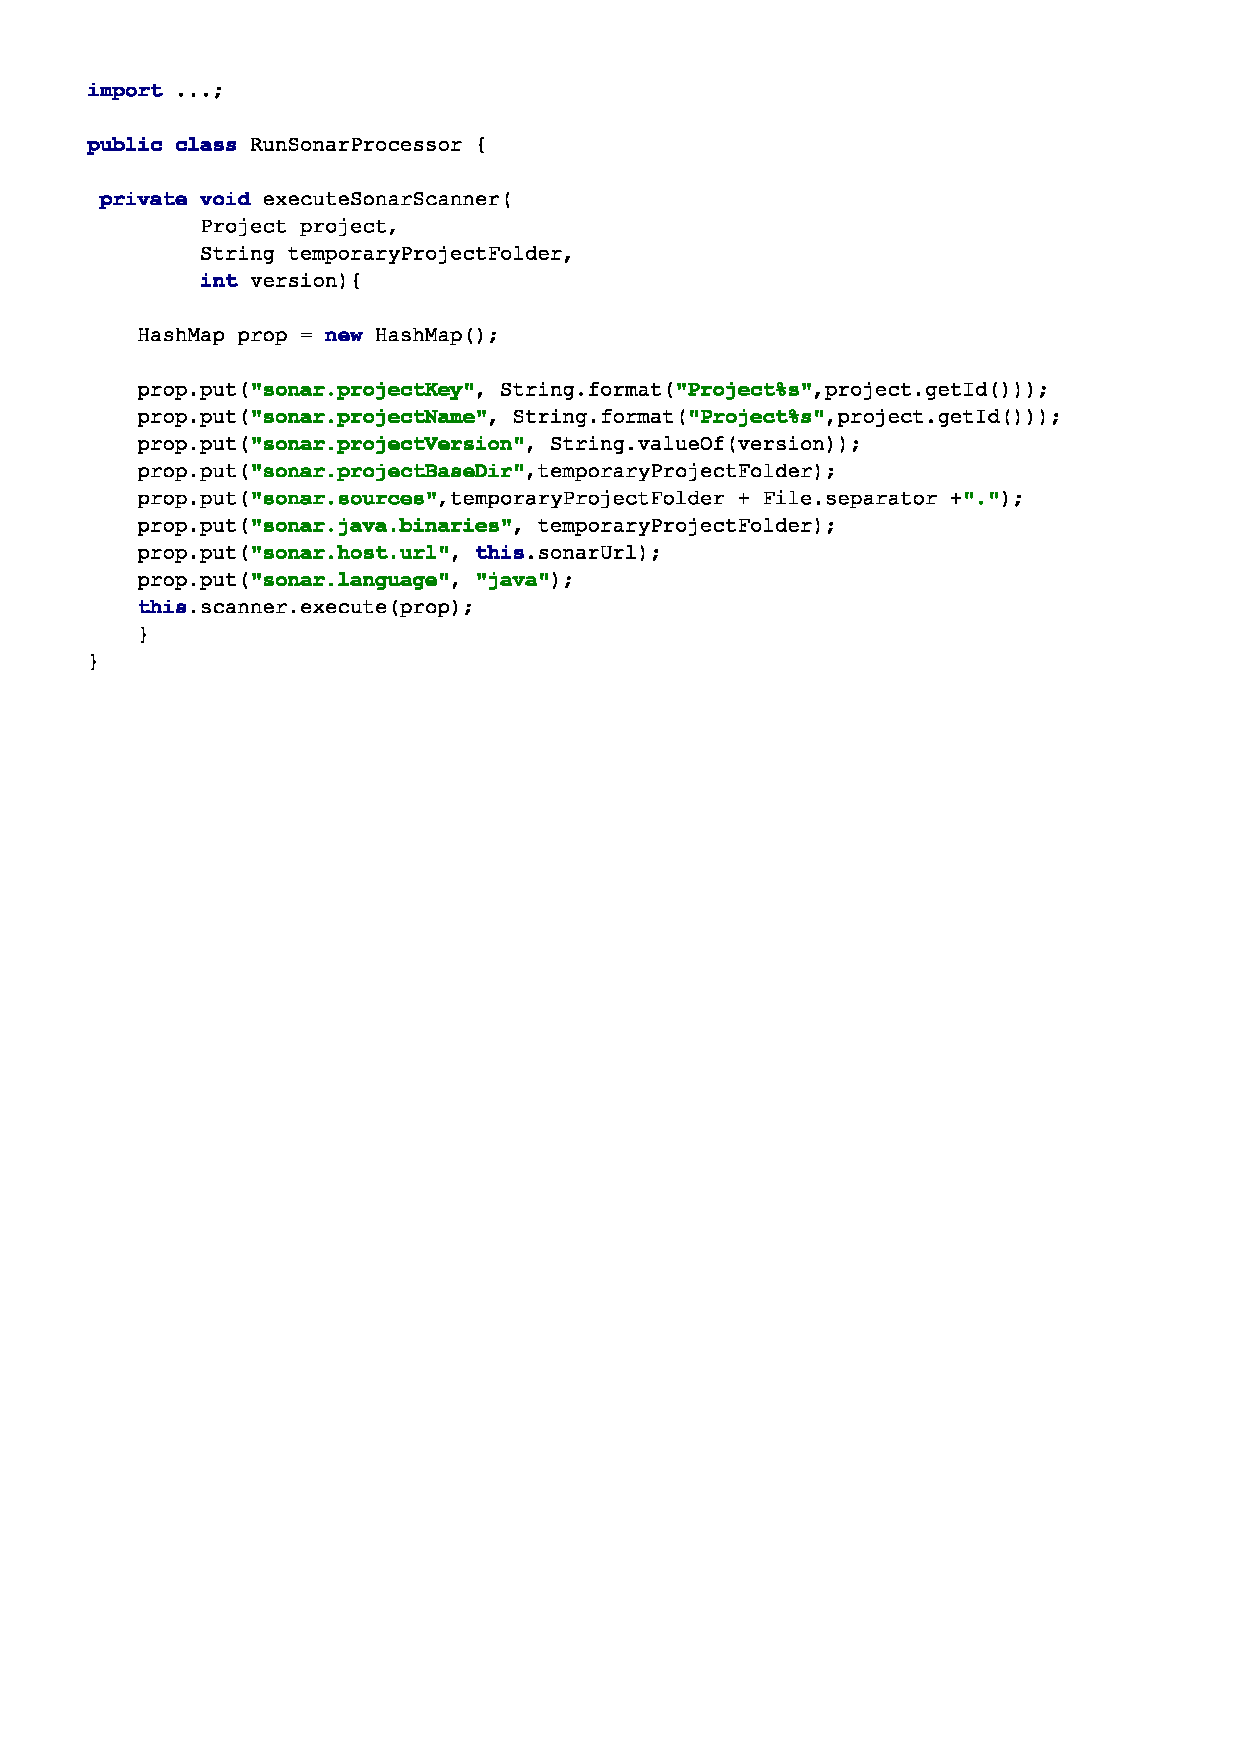
\includegraphics[trim={1cm 18cm 2.5cm 0},clip]{capitulo_estudo_caso/codigo_propriedades_sonar.pdf}} 
  \caption{Código responsável por criar a configuração para a execução do \textit{scanner} do SonarQube.}
  \label{fig:configuracao_sonar_scanner} 
\end{figure}


A Tabela \ref{table:metricas_sonar} contém as métricas que são disponibilizadas e que utilizamos nesta pesquisa.  Essas métricas ficam disponíveis no SonarQube automaticamente após a execução do \textit{scanner} em um projeto de software. Algumas dessas métricas são calculadas utilizando apenas o código-fonte da aplicação. Esse é o caso, por exemplo, da quantidade de arquivos, linhas de código, funções e classes. Entretanto, algumas das métricas disponibilizadas pelo SonarQube dependem de informações adicionais para serem calculadas. Esse é o caso  da Métrica $VIOLATIONS$. Essa métrica contém a quantidade de violações a regras de qualidade que foram encontradas no código-fonte. Essas regras ficam armazenadas no SonarQube e podem ser alteradas pelo usuário. Neste estudo de caso utilizamos o perfil de regras padrão disponibilizadas pelo SonarQube para a análise de qualidade de projetos java. Essas perfil é chamados de \textit{Sonar Way}\cite{arapidis2012sonar} e é baseado na metodologia de qualidade chamada \textit{sqale}\cite{letouzey2012sqale}.


\def\arraystretch{2.5}
\begin{longtable}{|c|c|}
\hline
\textbf{Métrica}                                       & \textbf{Descrição} \\ \hline
CODE\_SMELLS              	        &   \pbox{11cm}{Quantidade de trechos do código que contém uma violação a algum princípio fundamental da programação de sistemas\cite{suryanarayana2014refactoring}.}  \\  \hline
COGNITIVE\_COMPLEXITY        &   \pbox{11cm}{Um índice que indica o quão difícil é entender o código-fonte do projeto\cite{campbell2017cognitive}. }  \\ \hline
COMMENT\_LINES                     &  \pbox{11cm}{Quantidade de  linhas de comentários}   \\ \hline
COMMENT\_LINES\_DENSITY    &  \pbox{11cm}{Quantidade de linhas de comentários/(Linhas de código + Quantidade de linhas de comentários) * 100}   \\ \hline
COMPLEXITY                              &  \pbox{11cm}{Complexidade ciclomática do código-fonte\cite{mccabe1976complexity}. }   \\ \hline
DIRECTORIES                            &  \pbox{11cm}{Número de diretórios.}   \\ \hline
DUPLICATED\_LINES                 &  \pbox{11cm}{Linhas duplicadas}   \\ \hline
DUPLICATE\_LINES\_DENSITY  &  \pbox{11cm}{Linhas duplicadas / total de linhas * 100.}   \\ \hline
DUPLICATED\_BLOCKS              &  \pbox{11cm}{Número de blocos de códigos duplicados.}   \\ \hline
DUPLICATED\_FILES                 &  \pbox{11cm}{Número de arquivos duplicados.}   \\ \hline
FILES                                         &  \pbox{11cm}{Número de arquivos.}   \\ \hline
FUNCTIONS                               &  \pbox{11cm}{Número de funções.}   \\ \hline
NLOC                                         &  \pbox{11cm}{Número de linhas que contenham pelo menos um caractere que não seja um espaço, tabulação ou parte de um comentário.}   \\ \hline
SQALE\_DEBT\_RATIO              &  \pbox{11cm}{Razão entre o tempo estimado para resolver a dívida técnica do projeto e o tempo estimado que foi gasto para desenvolver o projeto. }   \\ \hline
SQALE\_RATING                       &  \pbox{11cm}{Uma classificação de 1 até 5 relativa ao nível de dívida técnica do projeto. Projetos com menos dívida técnica recebem a nota 1. }   \\ \hline
STATEMENTS                            &  \pbox{11cm}{Número de declarações no código-fonte.}   \\ \hline
VIOLATIONS                             &  \pbox{11cm}{Número de violações das regras de qualidade definidas no SonarQube.}   \\ \hline

\caption{Métricas extraídas dos projetos.}
\label{table:metricas_sonar}
\end{longtable}
\def\arraystretch{1}




\subsection{Medição da dívida técnica}

Conforme descrevemos no Capítulo \ref{cap:cap2}, existem diversos tipos de dívida técnica. Alguns desses tipos são de difícil medição devido às suas características subjetivas ou contextuais. A dívida técnica de tecnologia, por exemplo, acontece quando um projeto de software está utilizando uma tecnologia obsoleta. Porém, definir se uma tecnologia é ou não obsoleta é uma atividade normalmente subjetiva e sujeita às discordâncias. Já as dívidas técnicas de arquitetura dependem de uma análise contextual para serem medidas.  Esse tipo de dívida é descrito como uma violação a algum princípio ou regra pré-definido para como deve ocorrer a interação entre os componentes de um software. Acontece que parte dessas regras são específicas para o contexto no qual o software é desenvolvido. Isso acontece seja pelas necessidades do software sendo desenvolvido ou por aspectos relacionados aos desenvolvedores. No caso das dívidas técnicas arquiteturais, existem dificuldades de medição tanto por características contextuais quanto por aspectos subjetivos já que a aderência ou não de uma determinada arquitetura às expectativas de um desenvolvedor é algo subjetivo conforme boa parte dos arcabouços de avaliação de arquiteturas como é o caso do ATAM\cite{kazman2000atam}. Dessa forma, medir certos tipos de dívida técnica é uma tarefa difiícil e em alguns casos inviável de ser feita automaticamente. Por conta disso,  tivemos que limitar os tipos de dívida técnica avaliados neste estudo de caso. Isso foi feito por causa do nosso objetivo de medir quantitativamente e automaticamente o nível de dívida técnica dos projetos. Além disso, essa limitação foi realizada considerando os tipos de dívida técnica que a ferramenta SonarQube consegue medir. Com isso, o nível de dívida técnica que consideraremos em um projeto não será igual ao nível real já que serão considerados apenas alguns tipos de dívida.

A medição da dívida técnica é feita pelo SonarQube usando as regras definidas no perfil de qualidade utilizado no projeto. O nível de dívida técnica de um projeto é equivalente à soma do tempo estimado para alterar seu código-fonte de forma que todas as violações a regras de qualidade fossem eliminadas. Ou seja, o SonarQube escaneia o código-fonte do software em busca de violações. A cada violação encontrada, ele adiciona uma quantidade de tempo ao tempo total necessário para eliminar todas as dívidas técnicas do projeto. Após todo o código-fonte ser escaneado, o SonarQube  então armazena essa quantidade total de tempo. O nível de dívida técnica de um projeto é então calculado pela razão entre o tempo total estimado para desenvolver o software  e o tempo total que seria gasto para eliminar todas as dívidas técnicas. Esse cálculo é armazenado na métrica SQALE\_DEBT\_RATIO conforme mostrado na Tabela \ref{table:metricas_sonar}. A Tabela \ref{table:regras_sonar_way} apresenta algumas das regras de qualidade definidas no perfil padrão do SonarQube para a análise de projetos Java(\textit{Sonar Way}) e a quantidade de minutos estimados para eliminar cada uma das ocorrências de violações de cada regra.  

Forneceremos um exemplo de cálculo da dívida técnica utilizando o SonarQube. Para isso, analisaremos 2 projetos conforme a Tabela \ref{td_ratio_example}. O primeiro projeto tem 45.600 minutos de dívida técnica. Isso significa que após o SonarQube analisar todo o projeto, ele encontrou uma quantidade de dívidas que, somadas, levariam 45.600 minutos para serem resolvidas. Além disso, o  primeiro projeto possui  80.000 linhas de código-fonte. Com isso, o nível de dívida técnica do projeto 1 é calculado como $\frac{45.600}{80.000*m}$ sendo $m$ a quantidade de tempo que se estima necessária para escrever uma linha de código. O SonarQube usa como padrão 30 minutos para a variável $m$. No caso do projeto 1, o nível de dívida técnica foi calculado como 1,9\%. Isso significa que seriam gastos para eliminar a dívida técnica desse projeto 1,9\% do esforço necessário para construir o projeto inteiro. De acordo com Jesus et al. \cite{de2017technical}, um índice abaixo de 3\% é considerado baixo. Ou seja, o projeto 1 tem um nível baixo de dívida técnica.  Já o projeto 2, conforme a Tabela \ref{td_ratio_example} possui a mesma quantidade de dívida técnica medida em minutos. Entretanto, medido em número de linhas de código, o projeto 2 é muito menor do que o projeto 1. Isso fez com que o nível de dívida técnica do projeto 2 fosse calcado como 11,7\%. Ou seja, muito maior do que o projeto 1. Com isso, mesmo tendo o mesmo volume de dívida técnica que o projeto 1, de acordo com a estratégia de medição adotada, o projeto 2 é considerado pior do que o projeto 1 em termos de dívida técnica. Isso acontece porque o SonarQube
calcula o nível de dívida técnica de um projeto de uma forma proporcional ao seu tamanho.


\begin{table}[H]
\centering


\def\arraystretch{2.5}%
%\normalsize
\begin{tabular}{|l|l|l|l|l|}
\hline
        \textbf{Projeto}   & \textbf{Dívida técnica em minutos}  &  \textbf{Linhas de código} & \textbf{Cálculo} & \textbf{\textit{Debt Ratio}}\\ \hline
1 & 45600               & 80000         & $\frac{45600}{80000*m} $ &  1,9 \%    \\ \hline
2 & 45600               & 13000         & $\frac{45600}{80000*m} $ &  11,7  \%   \\ \hline
\end{tabular}
\caption{Exemplo de cálculo da dívida técnica com o SonarQube. A variável m representa o tempo necessário para escrever uma linha de código. O valor padrão no SonarQube é de 30 minutos. Adaptado de \cite{de2017technical}.}
\end{table}
\label{td_ratio_example}


\begin{table}[H]

\normalsize
\centering
\def\arraystretch{2.5}%
\begin{tabular}{|c|c|c|}

\hline
\textbf{Categoria}  & \textbf{Descrição} & \textbf{Minutos}  \\ \hline
Mutabilidade           &  \pbox{10cm}{Bloco de código duplicado.} & \pbox{1cm}{ 60 }  \\ \hline
Manutenção         &  \pbox{10cm}{Variável não usada.} & \pbox{1cm}{ 10 }  \\ \hline
Testabilidade           &   \pbox{10cm}{Complexidade ciclomática \cite{mccabe1976complexity} maior do que 10.} & \pbox{1cm}{ 11  }  \\ \hline
Reusabilidade        &   \pbox{10cm}{ Parâmetro usado como seleção em um método público. } & \pbox{1cm}{ 15  }  \\ \hline
Confiabilidade         &   \pbox{10cm}{A condição de um laço nunca será verdadeira.} & \pbox{1cm}{ 10  }  \\ \hline
Segurança                &   \pbox{10cm}{Comandos sendo enviados para o sistema operacional sem nenhuma validação } & \pbox{1cm}{ 30  }  \\ \hline
Portabilidade         &  \pbox{10cm}{Uso de métodos descontinuados.} & \pbox{1cm}{ 15  }  \\ \hline
Manutenção         &  \pbox{10cm}{Existência de código-fonte comentado.} & \pbox{1cm}{ 5 }  \\ \hline


\end{tabular}

\caption{Exemplos de regras para identificação de dívidas técnicas no SonarQube.}

\end{table}
\label{table:regras_sonar_way}
\def\arraystretch{1}%





\subsection{Limitações na medição da dívida técnica}


É possível identificar algumas limitações em relação a forma como o SonarQube realiza a medição do nível de dívida técnica de um projeto. A primeira delas é a falta de uma verificação empírica para a quantidade de minutos necessários para corrigir cada dívida. Por exemplo, de acordo com a Tabela \ref{table:regras_sonar_way}, remover um bloco de código duplicado levaria 60 minutos. Porém, não é possível encontrar na documentação da ferramenta nenhuma indicação de como esse valor foi definido. Com isso o tempo médio para refatorar o código-fonte e resolver esse problema pode ser muito maior ou muito menor do que 60 minutos. Outro ponto questionável é a lista de regras que são usadas para identificar dívidas técnicas na configuração padrão do SonarQube. Não há também na documentação da ferramenta qualquer menção a qual metodologia foi utilizada para criar essa lista. Inclusive, a capacidade de identificar dívidas técnicas por meio de algumas das regras utilizadas são claramente questionáveis. 

Apesar das limitações, o SonarQube tem sido usado efetivamente para a análise da dívida técnica em projetos de software, inclusive no contexto de pesquisas científicas. Uma das evidências da eficácia dessa ferramenta foi obtida por Marek et al.\cite{stochel2012value}. Nesse trabalho os autores realizaram um \textit{survey} com especialistas para que eles analisassem e indicasse o nível de dívida técnica de alguns projetos. Os dados obtidos foram então comparados com a medição realizada pelo SonarQube. As diferenças entre os dois resultados foram muito pequenas. Isso trouxe evidências de que a dívida técnica medida pelo SonarQube é tão precisa quanto aquela medida por especialistas.  Além disso, uma pesquisa realizada por Fontana et al.\cite{fontana2016tool} comparou algumas ferramentas que são capazes de calcular a dívida técnica de um projeto. Os autores chegaram à conclusão de que o SonarQube é a ferramenta mais precisa atualmente disponível. Apesar disso, conforme apontado por Fonta et al.\cite{fontana2016technical}, o índice de dívida técnica calculado pelo SonarQube não é apropriado para a análise individual de projetos. Ao invés disso, esse índice deve ser usado apenas para comparar projetos diferentes.  

\subsection{Divisão temporal do código}
\label{cap_experimento_divisao_temporal}
 
 
Todas as métricas obtidas do código-fonte dos projetos foram extraídas em 5 pontos diferentes na evolução do software.  Para realizar essa divisão utilizamos a quantidade de \textit{commits} de cada projeto. Por exemplo, se um projeto tem 1.000 \textit{commits}, fizemos a extração das métricas quando o projeto tinha apenas 200, depois quando tinha 400,600,800 e finalmente 1.000 \textit{commits}.  A Figura \ref{fig:codigo_conta_commits} exibe a porção de código no GitResearch responsável pela contagem dos \textit{commits} de um projeto. É possível notar que não basta apenas contar a quantidade de \textit{commits} já que, como mostrado na Figura \ref{fig:cap_experimento_exemplo_grafo_git_merge}, é possível que um \textit{commit} esteja envolvido em algum \textit{merge} e por isso possua mais de um pai. Para resolver esse problema e podermos navegar corretamente no grafo de \textit{commits}, nós consideramos apenas o primeiro pai encontrado conforme pode ser visto na linha 21 da Figura \ref{fig:cap_experimento_exemplo_grafo_git_merge}. O código responsável por executa o SonarQube em cada projeto é exibido na Figura \ref{fig:codigo_executa_sonar}.

 \begin{figure}[H]
  \centering
  \frame{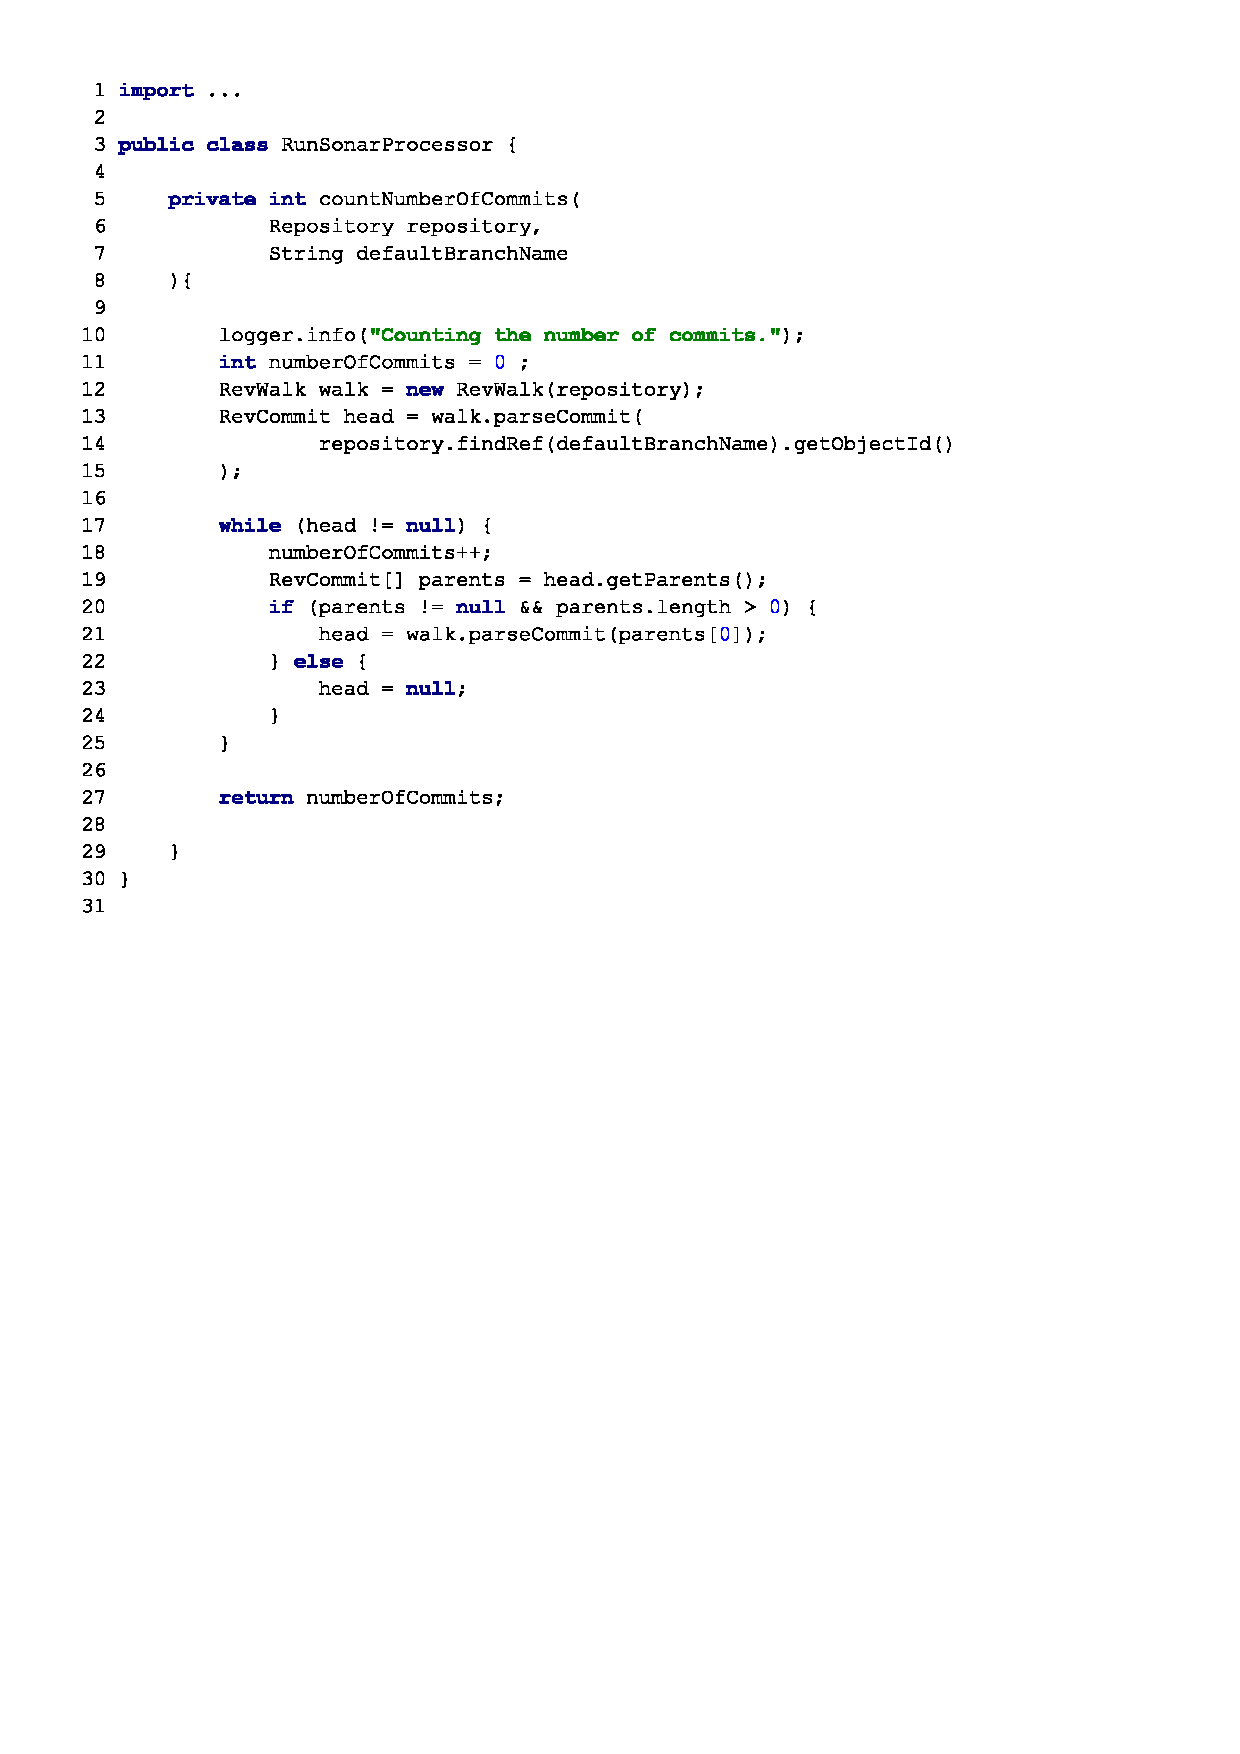
\includegraphics[trim={1cm 14cm 2.5cm 0},clip]{capitulo_estudo_caso/codigo_conta_commits.pdf}} 
  \caption{Código responsável por contar a quantidade de \textit{commits} de cada projeto.}
  \label{fig:codigo_conta_commits} 
\end{figure}

 \begin{figure}[H]
  \centering
  \frame{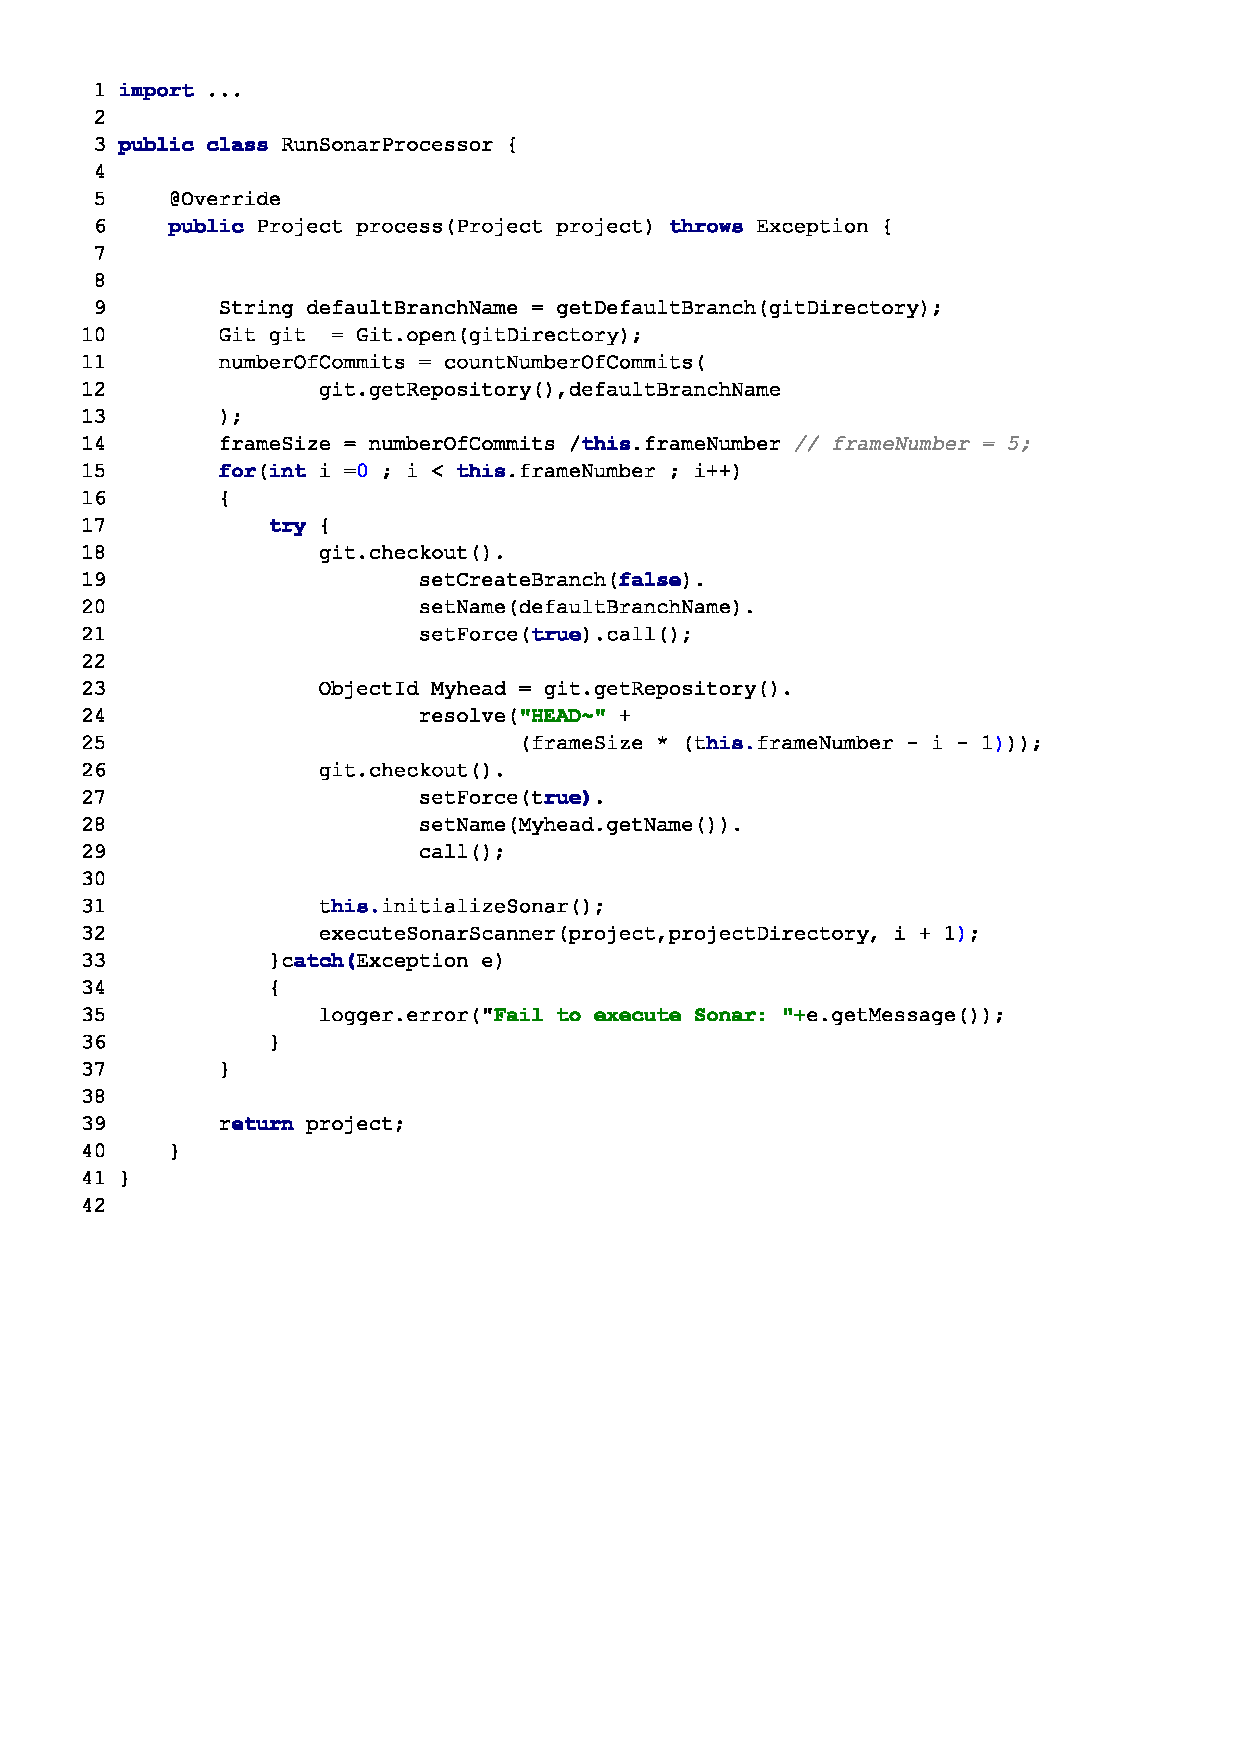
\includegraphics[trim={1cm 9cm 2.5cm 0},clip]{capitulo_estudo_caso/codigo_executa_sonar.pdf}} 
  \caption{Código responsável por executar o \textit{scanner} do SonarQube em cada projeto.}
  \label{fig:codigo_executa_sonar} 
\end{figure}
 


\section{Cálculo das variáveis de entrada do modelo}

Conforme descrito anteriormente, consideraremos a colaboração realizada em um projeto como a entrada em nossa estratégia de avaliação de produtividade. Se um projeto tem muita contribuição e pouca evolução, esse projeto será considerado improdutivo. Da mesma forma, se um projeto tem pouca contribuição, mas tem muita evolução, esse projeto será considerado produtivo. Conforme o Capítulo \ref{estimacao:juros}, a colaboração de um projeto será avaliada por meio de um índice que será calculado conforme a equação \ref{eq:cap_calculo_indice_colaboracao}. O valor $A(u)$ representa a assiduidade com o qual o colaborador $u$ contribuiu para o projeto $r$. Já o valor $Q(u)$ representa a qualidade do colaborador $u$. o Conjunto $u(R)$ contém todos os colaboradores que contribuíram no projeto $r$. A seguir descreveremos como foi calculado o $Ic$ de cada projeto.

\begin{equation}
\label{eq:cap_calculo_indice_colaboracao}
I_c(r) =  \sum_{u  \in u(R) } A(u) * Q(u)
\end{equation}





\subsection{Qualidade de colaboração}


Utilizamos a estratégia descrita no item \ref{cap_modelo_colaboracao_concreto} para calcular a qualidade de cada colaborador. Basicamente, para avaliar a qualidade realizamos uma análise no grafo com os relacionamentos entre colaboradores. Um colaborador será considerado de alta qualidade se ele possui muitos seguidores, contribuiu com projetos relevantes e colaborou com outros colaboradores de qualidade.  O cálculo de colaboração foi implementado na ferramenta GitResearch.  A Figura \ref{fig:codigo_calcula_pagerank} mostra uma das principais funções implementadas.  Nela é realizado o cálculo do \textit{pagerank} tanto dos colaboradores quanto dos projetos. As outras partes da estratégia foram implementadas com o auxílio dos dados disponibilizados pelo GHTorrent. A complexidade dessa implementação está na imensa quantidade de relacionamentos que precisam ser avaliados. Por exemplo, a relação seguir e ser seguido de todos os colaboradores que contribuíram com os projetos analisados gerou um grafo de aproximadamente 2 milhões de nós. Com isso, foi necessária a utilização de um hardware potente para que esses relacionamentos fossem calculados em um tempo viável para a realização do estudo de caso. 

 \begin{figure}[H]
  \centering
  \frame{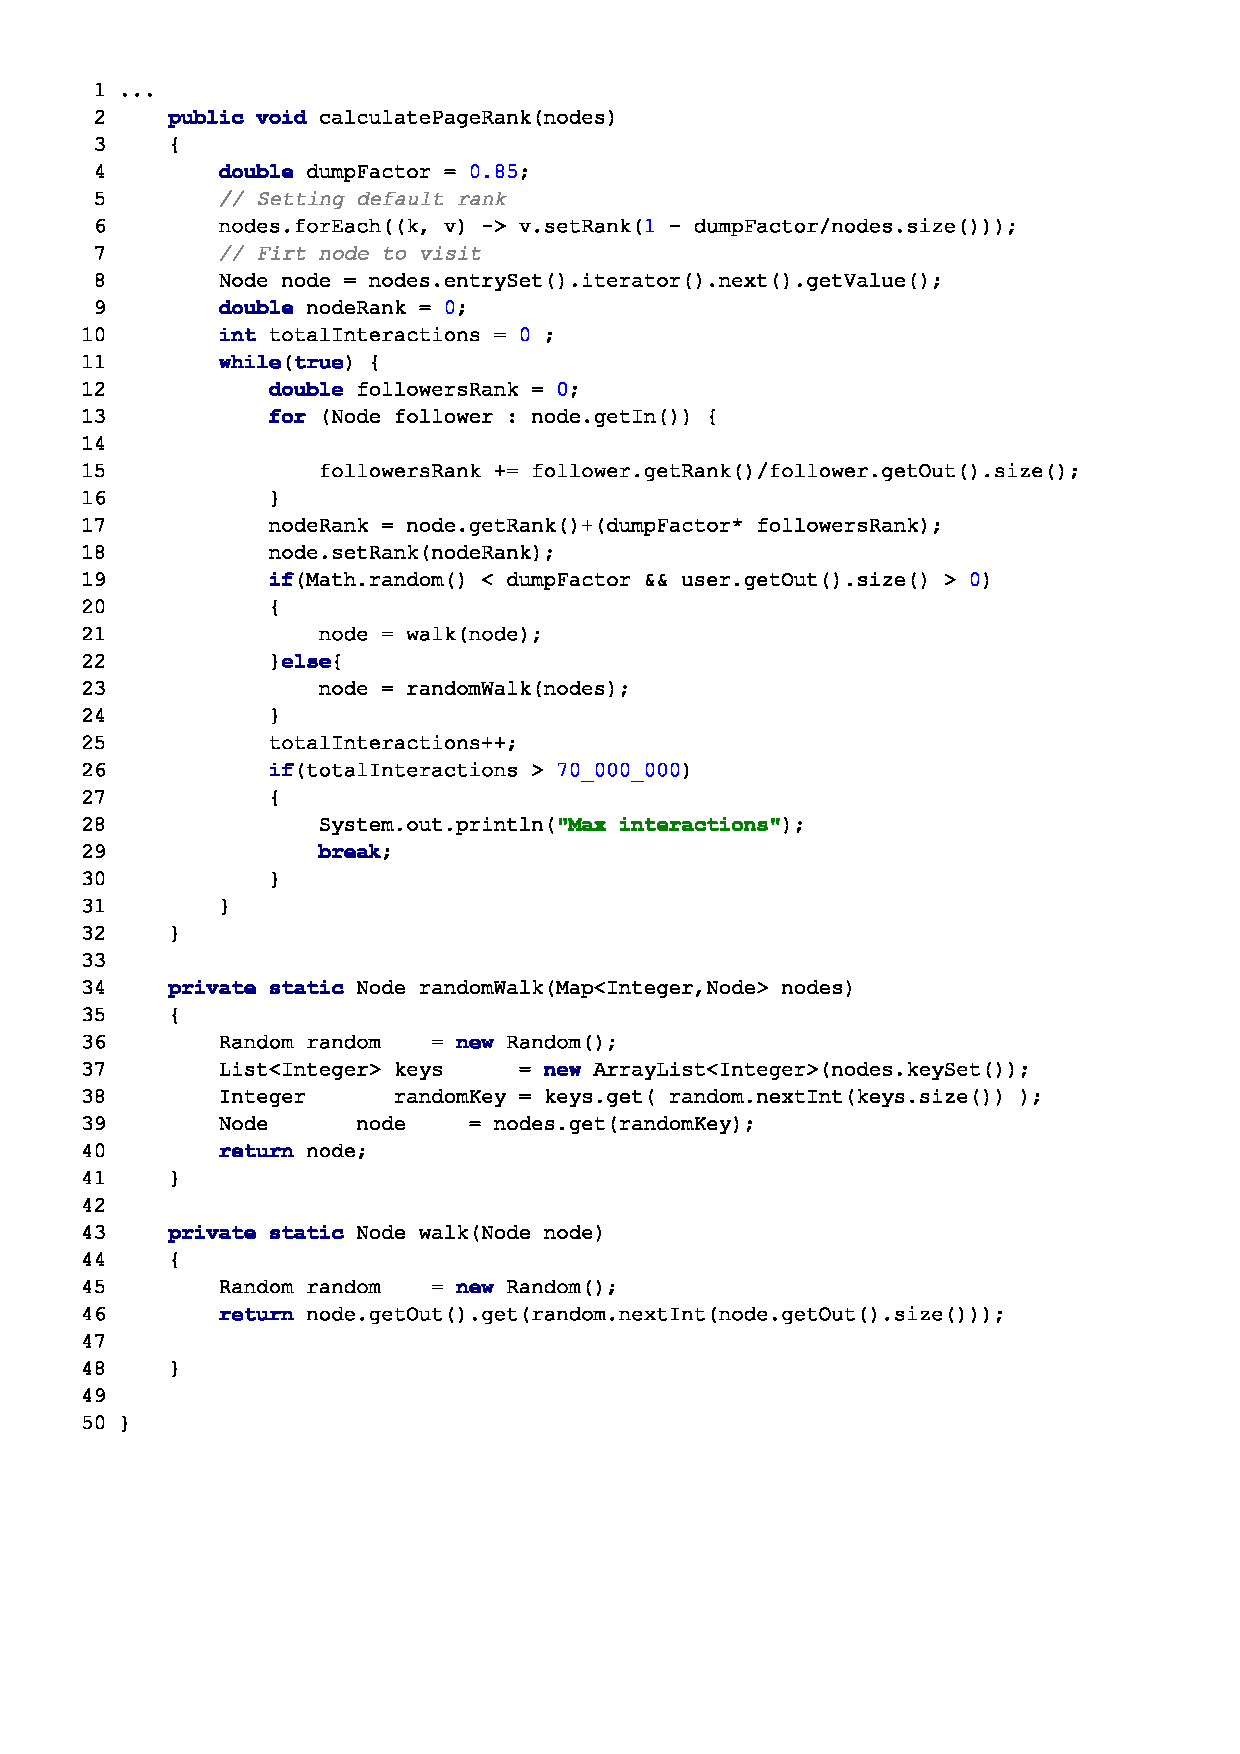
\includegraphics[trim={1cm 4.4cm 2.5cm 1cm},clip]{capitulo_estudo_caso/codigo_page_rank.pdf}} 
  \caption{Código responsável por calcular o pagerank.}
  \label{fig:codigo_calcula_pagerank} 
\end{figure}


\subsection{Assiduidade}

Analisando o banco de dados de commits disponibilizado pelo projeto GHTorrent até o mês de dezembro de 2017 pudemos calcular que a média de commits que um colaborador faz por dia em um mesmo projeto. O resultado desse cálculo foi: 1,16. Com isso, a assiduidade de um colaborador será calculada utilizando a equação \ref{eq:cap_calculo_assiduidade}. Nessa equação $D_r$ representa a quantidade de dias que um projeto possui desde o primeiro \textit{commit} até o último.  Já a variável $N(u_r)$ representa a quantidade de \textit{commits} que o colaborador $u$ realizou no projeto $r$. Se um colaborador tem uma média diária de \textit{commits} maior do que 1,16 , sua assiduidade no projeto será maior do que 1. Caso contrário, sua assiduidade será menor do que 1. Quanto mais \textit{commits} um colaborador fez em um projeto, maior será a sua assiduidade. 

\begin{equation}
\label{eq:cap_calculo_assiduidade}
A(u_r) =  \frac{N(u_r)}{1,16 * D_r}
\end{equation}


\section{Cálculo das variáveis de saída do modelo}

O cálculo das variáveis de saída foi realizado com facilidade já que foram escolhidas métricas que puderam ser obtidas diretamente dos dados no GHTorrent ou da análise feita pelo SonarQube. Foram utilizadas três métricas: linhas de código, estrelas e \textit{pull requests}.  A quantidade de linhas de código foi obtida por meio do SonarQube. Conforme a Tabela \ref{table:metricas_sonar}, essa métrica é uma das que a ferramenta disponibiliza após a análise de um projeto. Já a quantidade de estrelas e \textit{pull request} foram extraídas do GHTorrent. 

\section{Cálculo da produtividade dos projetos}

IN PROGRESS

\section{Estimação dos Juros}

IN PROGRESS

- Testar o número de violações como uma medida de dívida técnica ao invés de usar o SQALE INDEX.



\section{Dados obtidos}

Para avaliarmos os dados obtidos durante o estudo de caso realizaremos uma análise exploratória. Serão apresentadas diversas estatísticas e visualizações com o intuíto de fornecer um panomara a respeito das informações encontradas. Conforme explicado no Item \ref{cap_experimento_divisao_temporal}, todas as métricas foram obtidas em cinco pontos diferentes da evolução dos projeto. Entretanto,  quando não explicitado o contrário, todas as tabelas e gráficos são relativos aos valores mais atuais. Ou seja, foram criadas utilizando os dados da última leitura realizada. 



\subsection{Métricas}

A tabela \ref{tabela_sumario_metricas} apresenta um resumo com as principais medidas descritivas das métricas extraídas dos projetos. Existem alguns aspectos interessantes na Tabela \ref{tabela_sumario_metricas}. Um deles é a existência de métricas no qual o valor mínimo encontrado foi zero. Ao analisarmos esses projetos com valor zero nessas métricas, pudemos observar que isso ocorreu devido ao fato desses projetos terem sido descontinuados recentemente. Com isso, o código fonte na última leitura que realizamos, foi apagado ou drasticamente diminuído.  

Outra aspecto relevante da Tabela Tabela \ref{tabela_sumario_metricas} é o comportamento da métrica \textbf{sqale debt ratio}. Conforme a Tabela \ref{table:metricas_sonar}, essa métrica armazena a proporção entre o tamanho do software e a sua dívida técnica. Como podemos ver, essa métrica tem um desvio padrão próximo a 1. Isso indica que não há uma grande variação da proporção da dívida técnica entre os projetos.  Entretanto, o valor máximo é de 12,4. Isso é um indício da existência de \textit{outliers}. De acordo com Hawkins et al. \cite{hawkins1980identification}, um \textit{outlier} é um valor que se afasta demasiadamente dos demais de uma série ou é um valor medido incorretamente. Para verificarmos se não houve alguma falha na medição, realizamos uma análise dos 30 projetos com os maiores valores nessa métrica. Em todos os casos os valor medido anteriormente foi confirmado. Analisando o código-fonte desses projetos, chegamos as seguintes razões para o elevado nível de dívida técnica:

\begin{itemize}
\item A existência de códigos de teste com um nível de qualidade muito inferior ao restante do software.
\item A existência de arquivos e códigos descontinuados(\textit{deprecated}).
\item  Uma acentuada despreocupação dos colaboradores em seguir as boas práticas do desenvolvimento de software.
\end{itemize}


\begin{table}[H]
\scriptsize                 
\def\arraystretch{1.3}%
\centering
\begin{tabular}{|l|l|l|l|l|l|l|l|}
\hline
 &\textbf{Des. Padrão} & \textbf{Mín.}      & \textbf{1\textsuperscript{o} Quart.}  & \textbf{Mediana} & \textbf{Média}    & \textbf{3\textsuperscript{o}. Quart.}    & \textbf{Máx.}              \\ \hline
\textit{\textbf{CODE\_SMELLS }} & 10736,52     &0,0  &  637,2  & 1781,5 &  4897,7 &  4613,2 & 176454     \\ \hline
\textit{\textbf{COGNITIVE\_COMPLEXITY }} & 24376,92 & 0   & 1378    & 4176 & 12004 & 12174 & 440187  \\ \hline
\textit{\textbf{COMMENT\_LINES }} & 41883,15   & 5    & 1624      & 5083   &  17419   &  15624   & 690566     \\ \hline
\textit{\textbf{COMMENT\_LINES\_DENSITY}} & 8,274049    & 0,10  &  7,60    & 12,10     & 13,58    & 18,20    & 64,10  \\ \hline
\textit{\textbf{COMPLEXITY  }}   & 27665,5  & 0 & 2507  & 6244   & 15453  & 16386  & 413387 \\ \hline
\textit{\textbf{DIRECTORIES}} & 275,1348    & 1    & 34   & 79     & 169,2   & 183,8     & 3743,0    \\ \hline
\textit{\textbf{DUPLICATED\_LINES}}   & 44410,89    & 0 & 779  & 3155    & 15926     & 11737    & 577213      \\ \hline
\textit{\textbf{DUPLICATE\_LINES\_DENSITY}}   & 8,683636   & 0  & 2,400    & 5    & 7,367    & 8,90   & 97  \\ \hline
\textit{\textbf{DUPLICATED\_BLOCKS}}   & 3415,468   & 0  & 41   & 169    &   974,7  & 647,8    & 79718   \\ \hline
\textit{\textbf{DUPLICATED\_FILES  }}   & 363,5063    & 0  & 17    & 57     & 166,5    & 159    &  6078 \\ \hline
\textit{\textbf{FILES }}   & 1523,965    & 1  & 208    & 458,5     & 963,1   & 1056,2   & 20849  \\ \hline
\textit{\textbf{FUNCTIONS}}   & 14230,68    & 2  & 1468    & 3453     & 8226    & 8561    & 168295  \\ \hline
\textit{\textbf{NLOC}}   & 155979,5    & 30  & 15973   & 37429     & 91572    & 98373    & 1996351  \\ \hline
\textit{\textbf{SQALE\_DEBT\_RATIO}}   & 0,9809708    & 0,10  &  1,10    & 1,50    & 1,73    & 2,10    & 12,40   \\ \hline
\textit{\textbf{SQALE\_RATING}}   & 0,1121445    & 1  & 1    & 1     & 1,01   & 1    & 3  \\ \hline
\textit{\textbf{STATEMENTS }}   & 71565,78    &0  & 6401    & 15784     & 40319    & 43096    & 912227  \\ \hline
\textit{\textbf{VIOLATIONS }}   & 11374,37    & 0  & 708    & 1935   & 5319    & 5057    & 176844  \\ \hline

\end{tabular}
\caption{Sumário das medidas descritivas das métricas obtidas dos projetos.}
\end{table}
\label{tabela_sumario_metricas}


\subsection{Distruição dos projetos por tópicos}


Os projetos foram distribuidos em 30 tópicos após a aplicação do LDA. A Tabela \ref{table:tabela_quantidade_projetos_topicos} e a Figura \ref{fig:projetos_por_topicos} apresentam a quantidade de projetos em cada um dos tópicos. Podemos observar que não houve uma distruição uniforme dos projetos em cada tópico. Alguns tópicos como o 13 tiveram uma quantidade maior de projetos. Enquanto isso, alguns tópicos como o 28 e 10 tiveram uma quantidade significativamente menor de projetos. Existem algumas razões para essa variação:

\begin{itemize}
\item A existência de alguns assuntos que genuinamente possuem mais projetos relacionados no GitHub. Esse é o caso, por exemplo, do tópico 9 que é o segundo maior tópico obtido. Na Tabela \ref{table:topicos_lda} podemos ver as palavras presentes nesse tópico e com isso, inferir que os projetos presentes nele são relacionados a aplicações para a internet. Isso explica a quantidade maior de projetos já que esse é um domínio popular. 
\item As definiciências na utilização do LDA para a categorização de projetos de software. No caso do tópico 13, uma das possíveis razões para o seu alto número de projetos é a quantidade de palavras muito comuns que ele possui. De acordo com a Tabela \ref{table:topicos_lda}, as duas primeiras palavras desse tópico são \textit{issue} e \textit{contribution}. Essas palavras são demasiadamente comuns na descrição de projetos de software livre. Isso fez com que o tópico 13 fosse o tópico com o maior número de projetos.
\end{itemize} 


\begingroup
\begin{longtable}{|l|r|}

\hline
Tópico & Quantidade de projetos\\
\hline
Tópico 1 & 38\\
\hline
Tópico 10 & 10\\
\hline
Tópico 11 & 35\\
\hline
Tópico 12 & 35\\
\hline
Tópico 13 & 259\\
\hline
Tópico 14 & 35\\
\hline
Tópico 15 & 32\\
\hline
Tópico 16 & 64\\
\hline
Tópico 17 & 18\\
\hline
Tópico 18 & 22\\
\hline
Tópico 19 & 20\\
\hline
Tópico 2 & 32\\
\hline
Tópico 20 & 64\\
\hline
Tópico 21 & 109\\
\hline
Tópico 22 & 80\\
\hline
Tópico 23 & 194\\
\hline
Tópico 24 & 65\\
\hline
Tópico 25 & 42\\
\hline
Tópico 26 & 25\\
\hline
Tópico 27 & 63\\
\hline
Tópico 28 & 10\\
\hline
Tópico 29 & 48\\
\hline
Tópico 3 & 114\\
\hline
Tópico 30 & 20\\
\hline
Tópico 4 & 26\\
\hline
Tópico 5 & 19\\
\hline
Tópico 6 & 66\\
\hline
Tópico 7 & 42\\
\hline
Tópico 8 & 11\\
\hline
Tópico 9 & 216\\
\hline
\caption{Quantidade de projetos por tópico.}
\end{longtable}
\label{table:tabela_quantidade_projetos_topicos}
\endgroup





Para facilitar a visualização do comportamento dos dados  realizamos um agrupamento dos tópicos por domínio conforme mostrado na Tabela \ref{table_cap_estudo_topicos_dominios}. Esse agrupamento foi feito observando as palavras de cada um dos tópicos e analisando alguns dos projetos de cada tópico. Foram identificados 7 domínios: Aplicação, Gerenciamento de Dados, Ferramenta, Arcabouço, Mddleware, Biblioteca e Outro. Todos os projetos que não puderam ser classificados foram colocados no domínio Outro. A Figura \ref{fig:projetos_por_dominio} apresenta a distrubuição dos projetos dentro dos 7 domínios. É possível nota que houve uma distribuição mais uniforme dos projetos quando é realizado o agrupamento dos tópicos em domínios. 



 \begin{figure}[H]
  \centering
  \frame{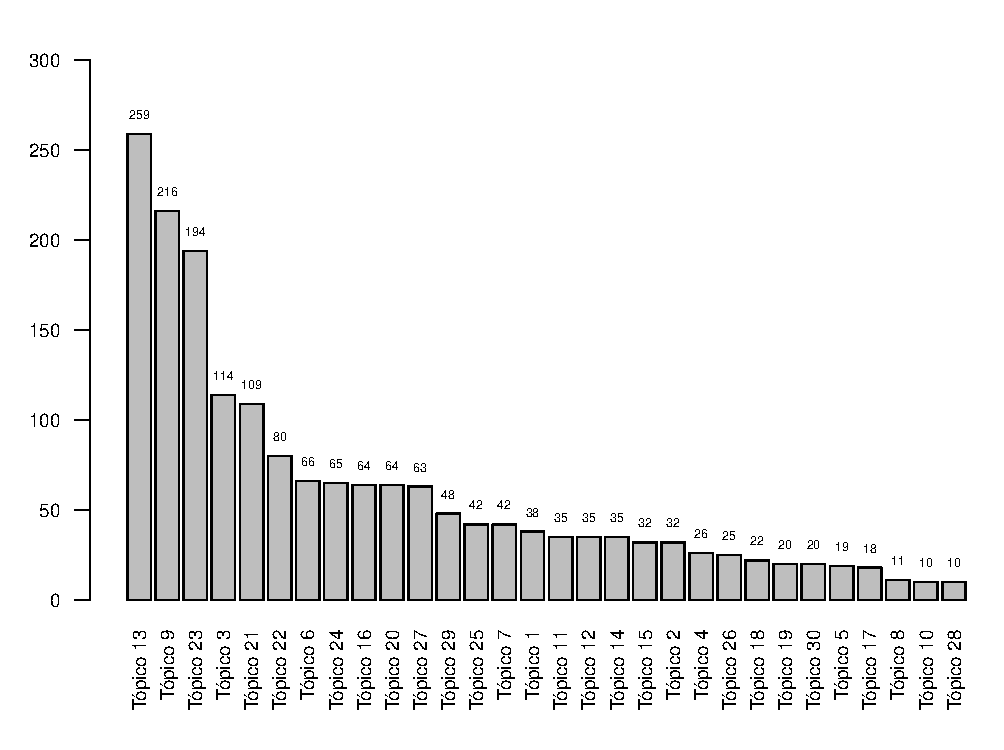
\includegraphics[trim={0cm 0cm 0cm 0cm},clip]{capitulo_estudo_caso/analise_exploratoria/projetos_por_topicos.pdf}} 
  \caption{Quantidade de projetos por tópico do LDA.}
  \label{fig:projetos_por_topicos} 
\end{figure}

\begin{table}[H]
\small 
\def\arraystretch{3}% 
\begin{tabular}{|l|l|l|l|}
\hline
\textbf{Domínio}       & \pbox{1cm}{\textbf{Tópicos}}  &  \pbox{5cm}{\textbf{Descrição}}                                     &  \pbox{4cm}{\textbf{Exemplos}}                               \\ \hline
Aplicação              & \pbox{1cm}{1, 4, 9, 10, 17, 22, 28} &  \pbox{5cm}{Programas voltados para o usuário final.}                &  \pbox{4cm}{Morphium, XPrivacy, Mule, SilenceIM}              \\ \hline
Gerenciamento de dados & \pbox{2cm}{2, 5, 12, 21, 24, 25}   &  \pbox{5cm}{Aplicações para processamento e gerenciamento de dados.} &  \pbox{4cm}{Asterixdb, Cassandra, Hive, Hibernate-ogm}          \\ \hline
Ferramenta             & \pbox{1cm}{3, 23, 30}           &  \pbox{5cm}{Ferramentas de desenvolvimento.}                         &  \pbox{4cm}{Cloudify, Kotlin-eclipse, Bitcoinj, Pentaho-kettle} \\ \hline
Arcabouço              & \pbox{1cm}{6, 18, 19, 20, 27}     &  \pbox{5cm}{Arcabouços para o desenvolvimento de software.}          &  \pbox{4cm}{Spring-cloud-commons, Guava, arquillian-cube}    \\ \hline
Middleware             & \pbox{1cm}{7, 14}              &  \pbox{5cm}{Aplicações voltadas para a infraestrutura.}              &  \pbox{4cm}{Docker-maven-plugin, s3proxy, aws-mock}          \\ \hline
Biblioteca             & \pbox{1cm}{8, 15, 16, 26}        & \pbox{5cm}{Bibliotecas de códigos.}                                 &  \pbox{4cm}{Tnt4j, Swagger-codegen, java-client-api}         \\ \hline
Outro                  & \pbox{1cm}{11, 13, 29}          & \pbox{5cm}{Não puderam ser classificados.}                          &  \pbox{4cm}{Abstools, react-native, RxJava, vraptor4}        \\ \hline
\end{tabular}
\caption{Tópicos agrupados em domínios.}
\end{table}
\label{table_cap_estudo_topicos_dominios}




 \begin{figure}[H]
  \centering
  \frame{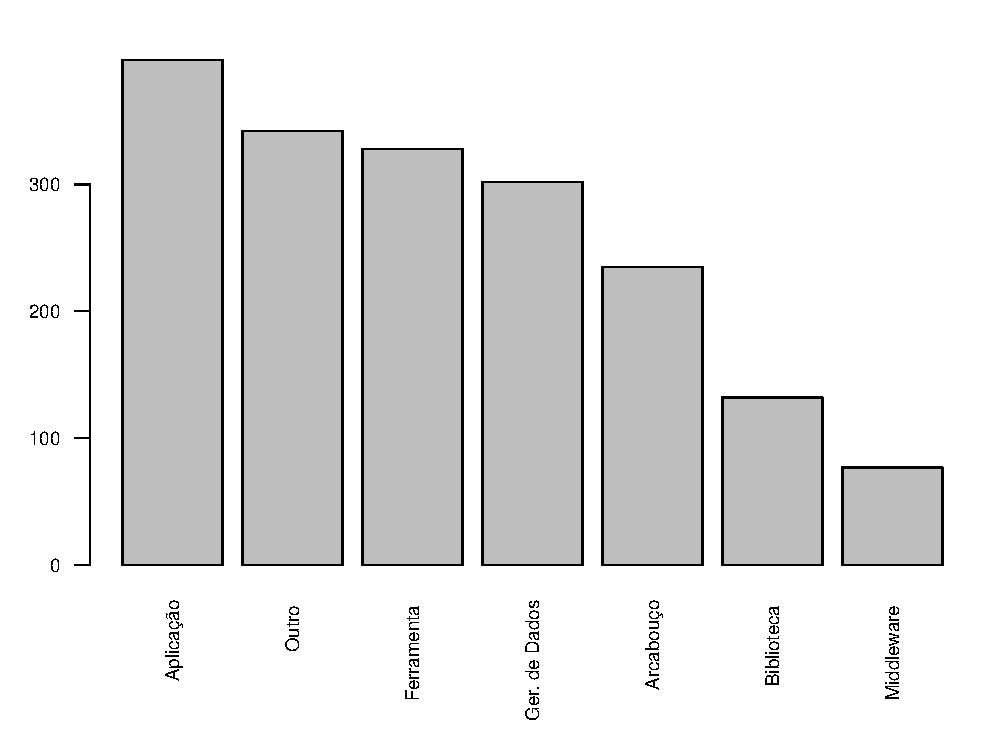
\includegraphics[trim={0cm 0cm 0cm 0cm},clip]{capitulo_estudo_caso/analise_exploratoria/projetos_por_dominio.pdf}} 
  \caption{Quantidade de projetos por domínio.}
  \label{fig:projetos_por_dominio} 
\end{figure}


\subsection{Dívida técnica}

A Figura \ref{fig:boxplot_divida_tecnica} apresenta um \textit{boxplot} a respeito da distribuição da dívida técnica em todos os projetos do estudo de caso. Conforme pode ser visto, a mediana se aproxima de 1,5. Isso vai de encontro a resultados de pesquisas anteriores onde o valor da mediana era próximo de três\cite{de2017technical}. As Figura \ref{fig:divida_por_topico} e \ref{fig:divida_por_dominio} apresentam \textit{boxplots} com a distribuição do valor da dívida técnica dos projetos agrupados por tópicos e domínios, respectivamente. 


 \begin{figure}[H]
  \centering
  \frame{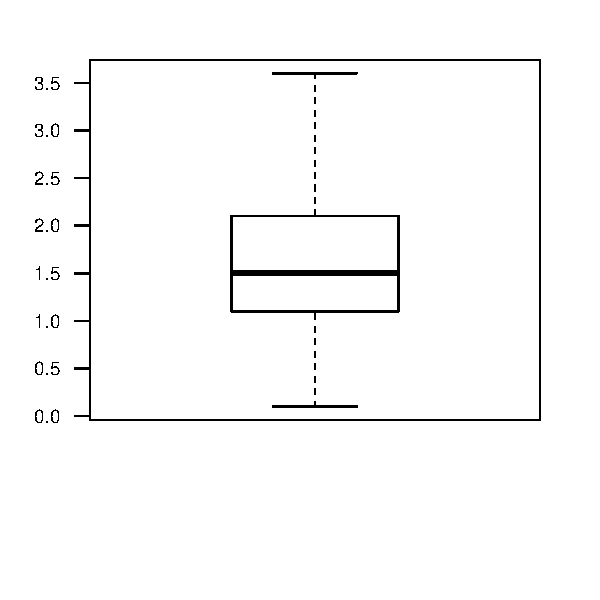
\includegraphics[trim={0cm 2cm 0cm 0cm},clip]{capitulo_estudo_caso/analise_exploratoria/divida_tecnica_sozinha.pdf}} 
  \caption{Dívida técnica.}
  \label{fig:boxplot_divida_tecnica} 
\end{figure}

 \begin{figure}[H]
  \centering
  \frame{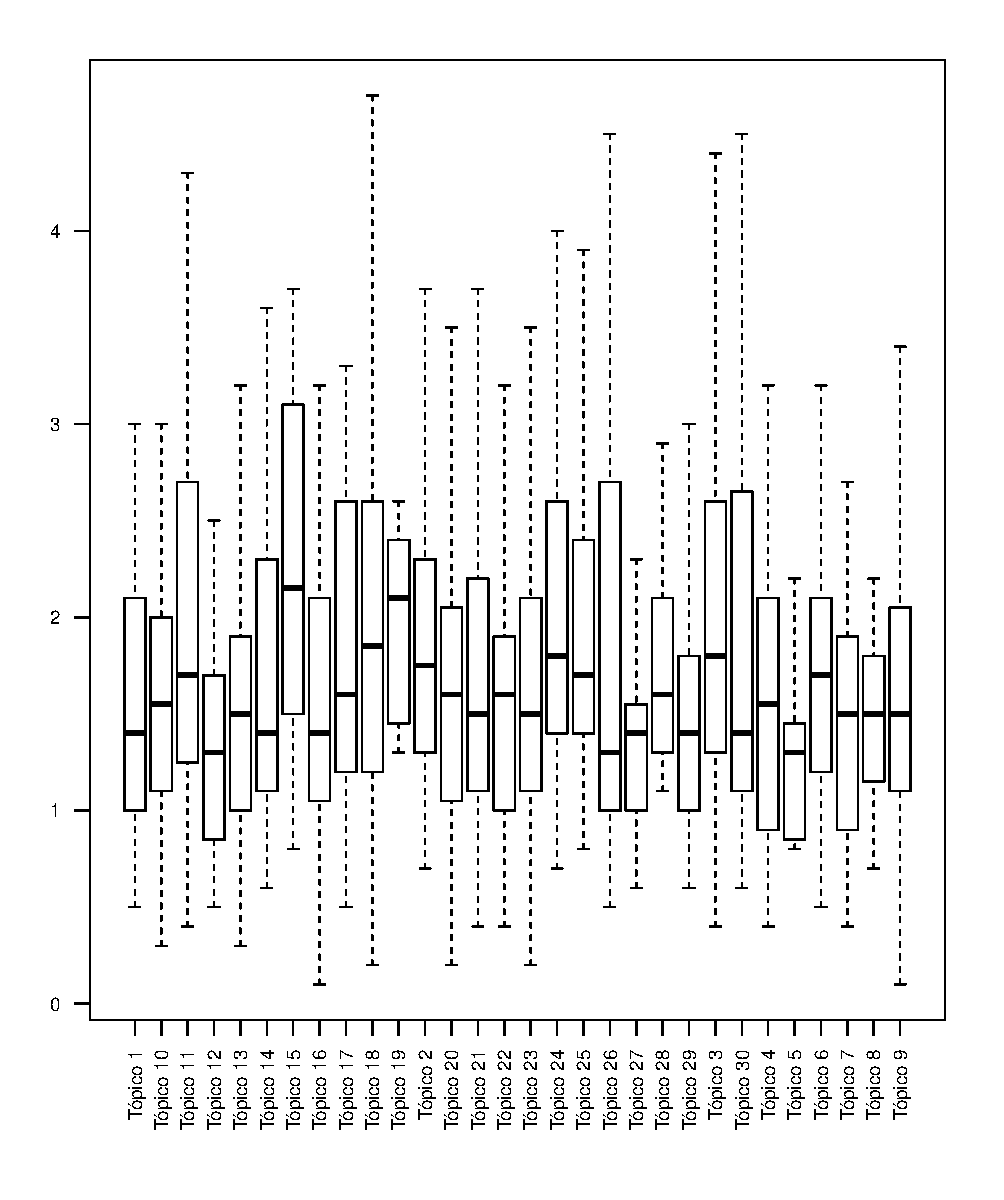
\includegraphics[trim={0cm 0cm 0cm 0cm},clip]{capitulo_estudo_caso/analise_exploratoria/divida_tecnica_por_topico.pdf}} 
  \caption{Dívida técnica por tópico.}
  \label{fig:divida_por_topico} 
\end{figure}

 \begin{figure}[H]
  \centering
  \frame{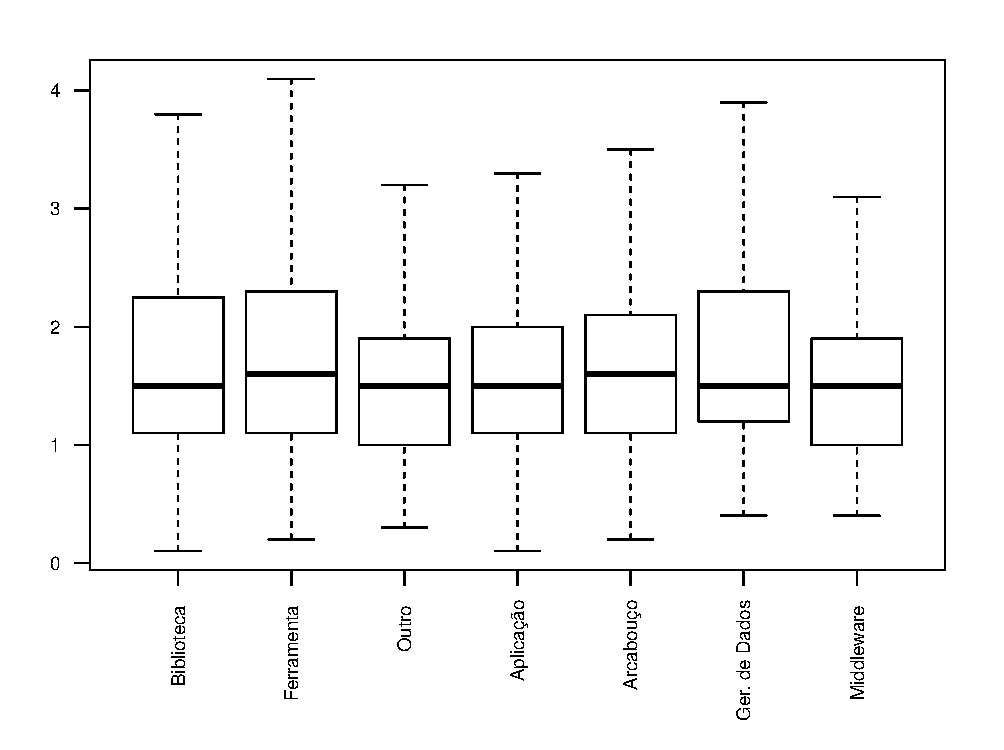
\includegraphics[trim={0cm 0cm 0cm 0cm},clip]{capitulo_estudo_caso/analise_exploratoria/divida_tecnica_por_dominio.pdf}} 
  \caption{Dívida técnica por domínio.}
  \label{fig:divida_por_dominio} 
\end{figure}


Na Figura \ref{fig:histograma_leitura_divida} é apresentado um histograma, com a quantidade de projetos por intervalo de dívida técnica, para cada leitura realizada. 

 \begin{figure}[H]
  \centering
  \frame{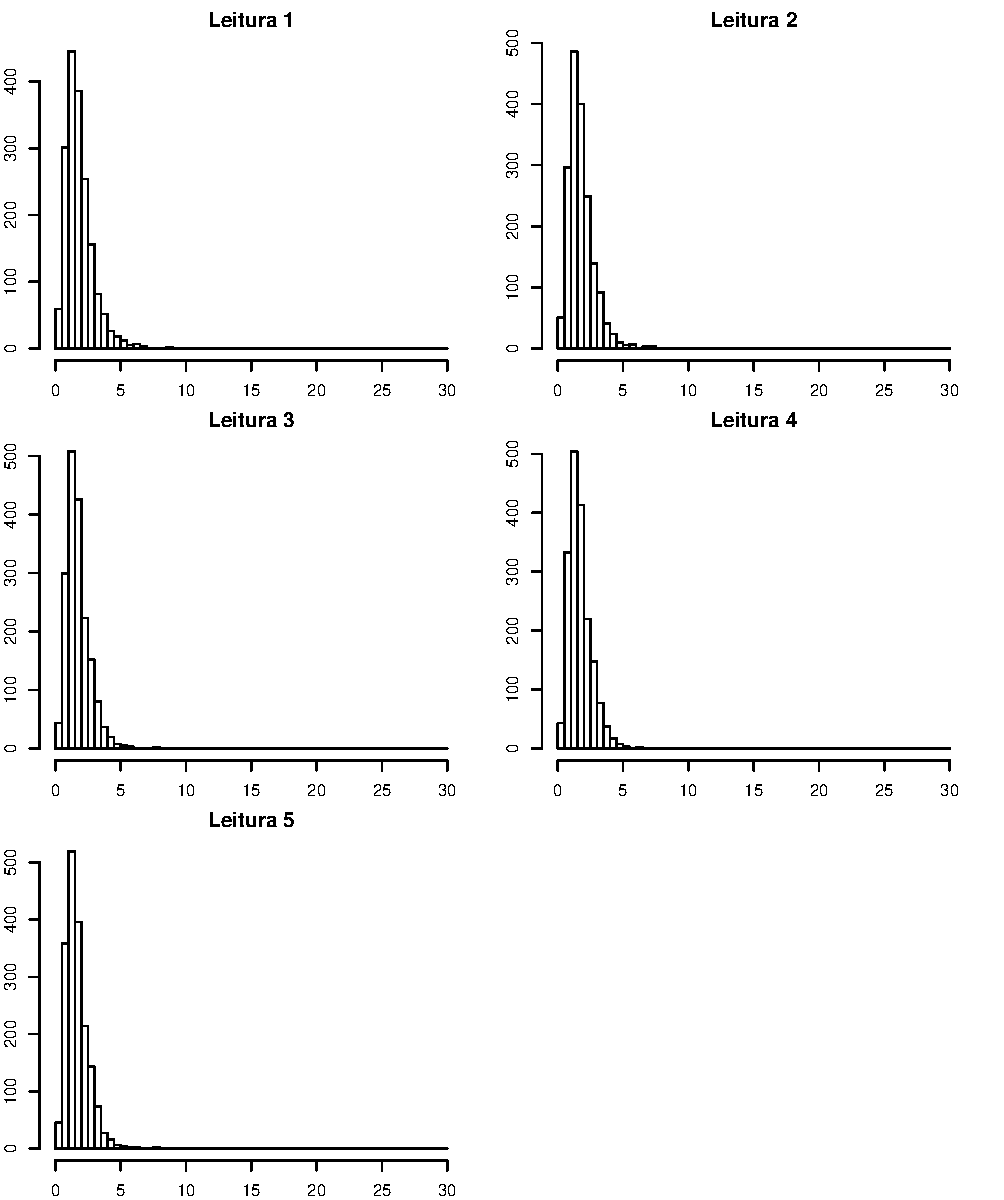
\includegraphics[trim={0cm 0cm 0cm 0cm},clip]{capitulo_estudo_caso/analise_exploratoria/histograma_divida_leitura.pdf}} 
  \caption{Dívida técnica por domínio.}
  \label{fig:histograma_leitura_divida} 
\end{figure}


Por termos feitos cinco leituras em períodos diferentes da evolução dos projetos, podemos analisar a evolução da dívida técnica nos mesmos. A Figura \ref{fig:evolucao_por_dominio} apresenta a evolução da dívida técnica nos projetos agrupados por domínio. É possível notar que há predominantemente uma tendência de queda. Ou seja, a medida que os projetos evoluem, o nível da dívida técnica cai. Entretanto, essa variação temporal é pequena.  Um exemplo são os projetos do domínio \textbf{aplicação}. Inicialmente a média da dívida técnica desses projetos foi de aproximadamente 1,9. Entretanto, com o passar do tempo, essa média caiu para 1,65. 



 \begin{figure}[H]
  \centering
  \frame{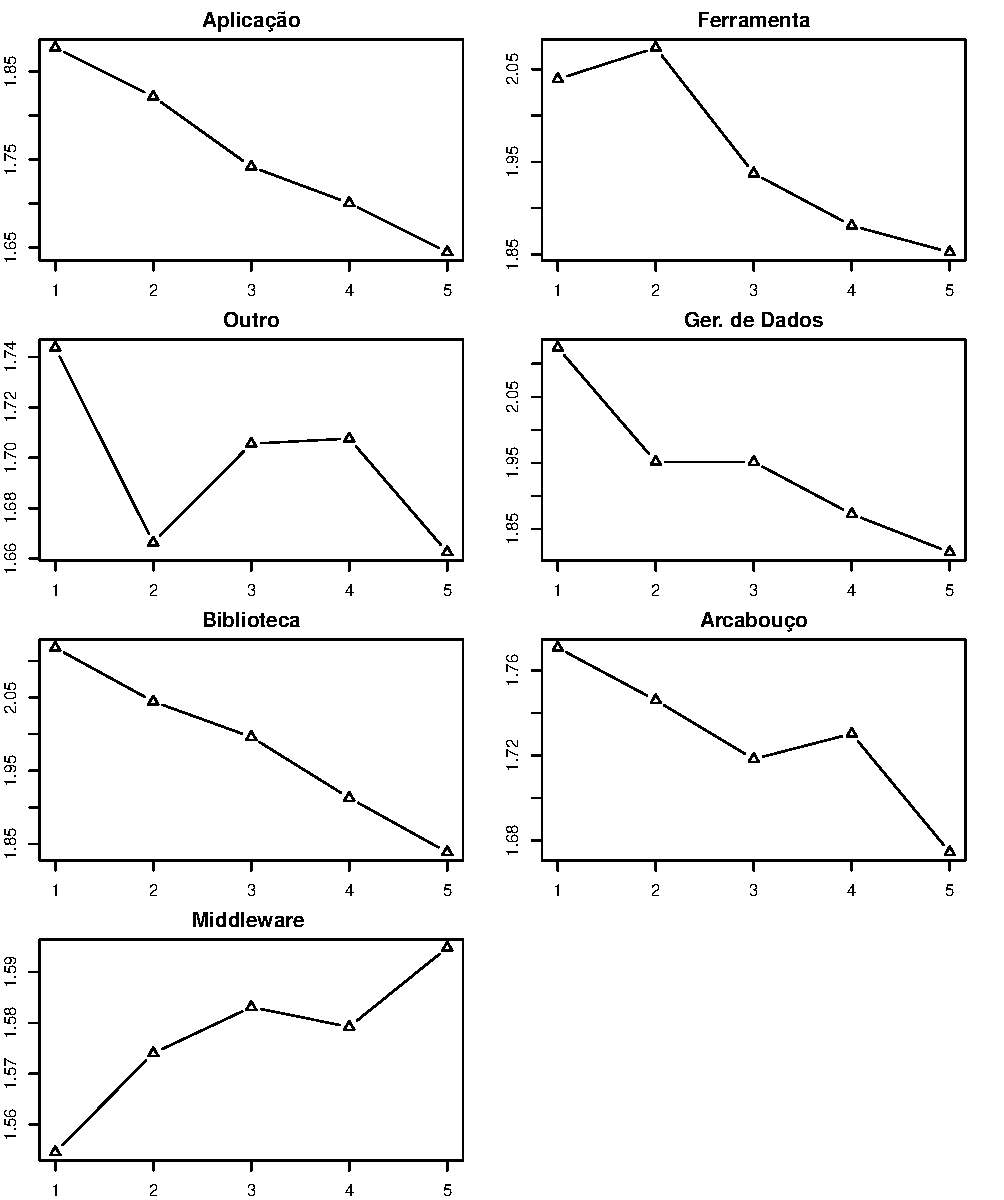
\includegraphics[trim={0cm 0cm 0cm 0cm},clip]{capitulo_estudo_caso/analise_exploratoria/evolucao_divida_dominio.pdf}} 
  \caption{Evolução da dívida técnica por domínio.}
  \label{fig:evolucao_por_dominio} 
\end{figure}



\subsection{Tamanho}

A Figura \ref{fig:histograma_nloc} apresenta um histograma com o número de projetos por faixa de tamanho. É possível verificar que grande parte dos projetos tem menos do que quinhentas mil linhas de código-fonte. Porém, existem alguns projetos acentuadamente maiores e que ultrapassam as cem mil linhas. As Figuras \ref{fig:histograma_nloc} e \ref{fig:linhas_codigo_dominio} apresentam \textit{boxplots} com a distribuição da quantidade de linhas de código agrupadas por tópicos e domínios respectivamente. Já a Figura \ref{fig:evolucao_linhas_codigo_dominio} apresenta a evolução da quantidade de linhas de código entre as leituras realizadas. Como esperado, há uma tendência de crescimento já que a medida que o software evoluiu, mais linhas de código são inseridas. 


 \begin{figure}[H]
  \centering
  \frame{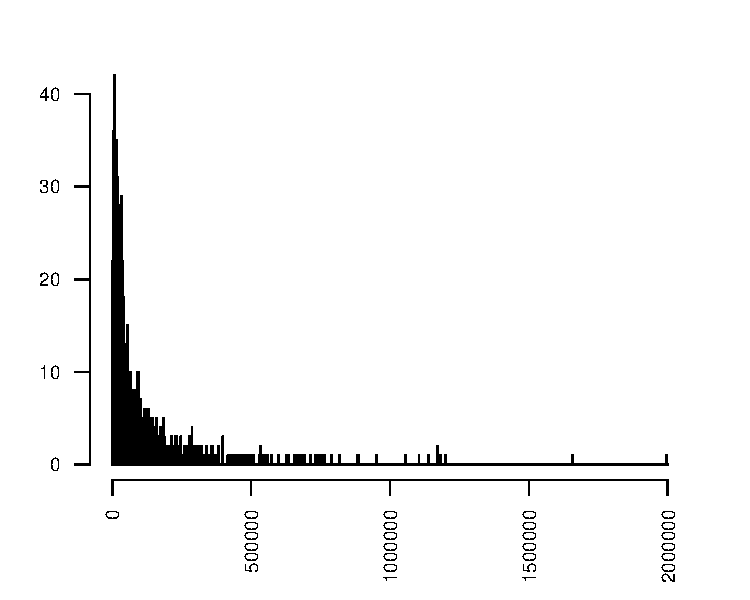
\includegraphics[trim={0cm 0cm 0cm 0cm},clip]{capitulo_estudo_caso/analise_exploratoria/histograma_nloc.pdf}} 
  \caption{Frequência de projetos por intervalo de número de linhas de código.}
  \label{fig:histograma_nloc} 
\end{figure}



 \begin{figure}[H]
  \centering
  \frame{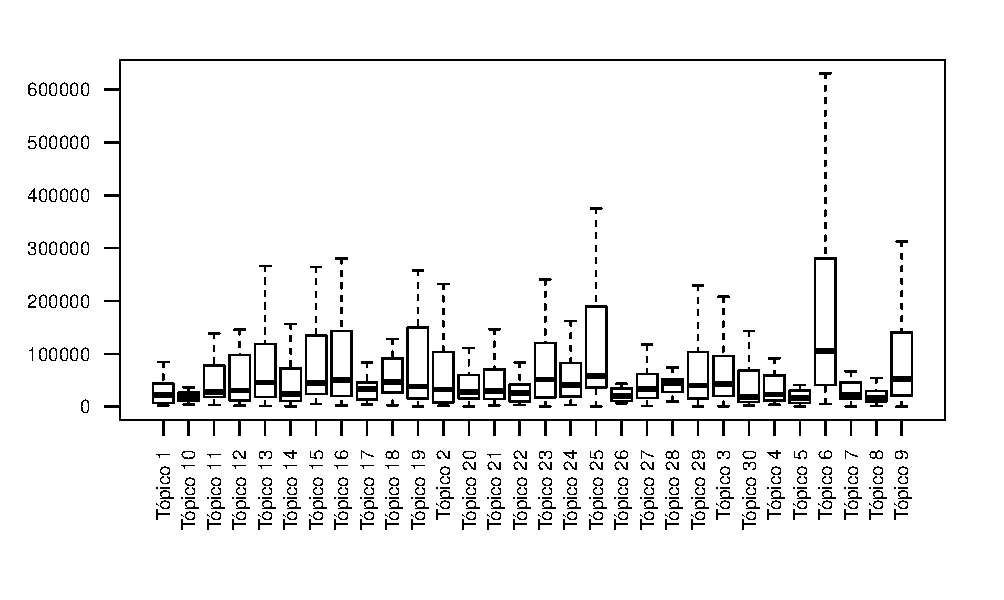
\includegraphics[trim={0cm 0cm 0cm 0cm},clip]{capitulo_estudo_caso/analise_exploratoria/linhas_de_codigo_por_topico.pdf}} 
  \caption{Dívida técnica por domínio.}
  \label{fig:linhas_codigo_topico} 
\end{figure}

 \begin{figure}[H]
  \centering
  \frame{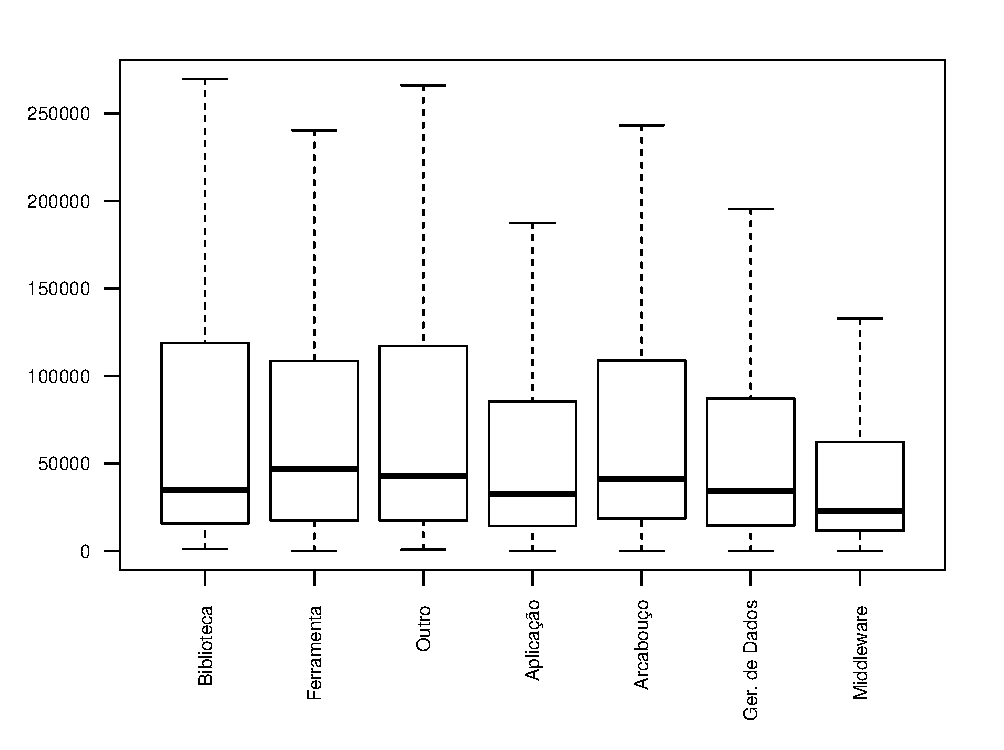
\includegraphics[trim={0cm 0cm 0cm 0cm},clip]{capitulo_estudo_caso/analise_exploratoria/linhas_de_codigo_por_dominio.pdf}} 
  \caption{Dívida técnica por domínio.}
  \label{fig:linhas_codigo_dominio} 
\end{figure}


 \begin{figure}[H]
  \centering
  \frame{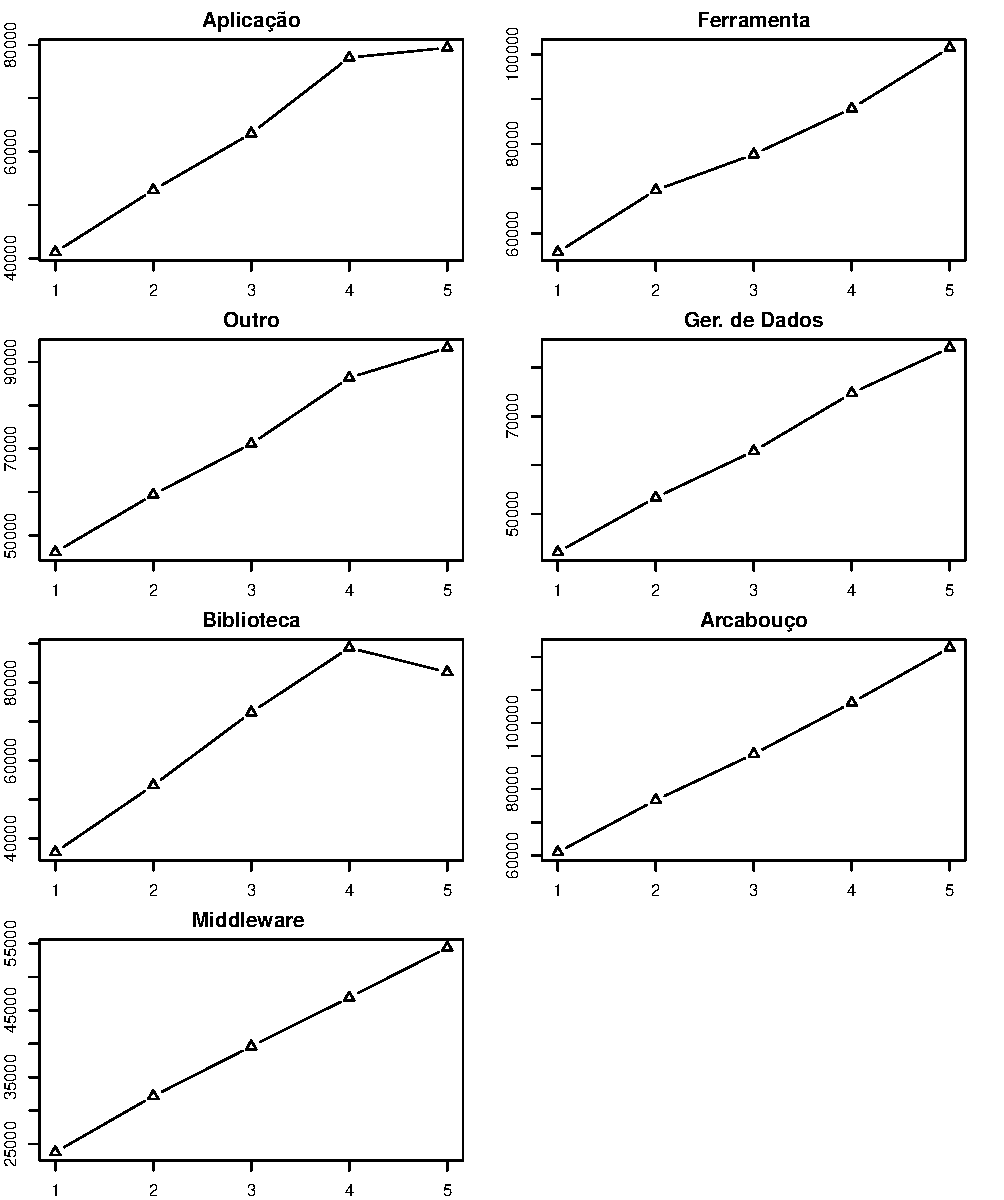
\includegraphics[trim={0cm 0cm 0cm 0cm},clip]{capitulo_estudo_caso/analise_exploratoria/evolucao_linhas_de_codigo_dominio.pdf}} 
  \caption{Dívida técnica por domínio.}
  \label{fig:evolucao_linhas_codigo_dominio} 
\end{figure}


\subsection{Correlações entre a dívida técnica e as métricas de tamanho}

Nas Figuras \ref{fig:correlacao_divida_linhas_codigo},  \ref{fig:correlacao_divida_watchers} e \ref{fig:correlacao_divida_pull_request} foram exibidas as correlações entre a dívida técnica e as variáveis linhas de código, \textit{watchers} e \textit{pull requests}, respectivamente. Conforme pode ser notado, apenas há indício de correlação com a variável linhas de código. Ainda assim, essa correlação, medida de forma geral, sem separação por domínios, é de apenas 0,1164773  com \textit{p-value} de 0,0000006545. 

 \begin{figure}[H]
  \centering
  \frame{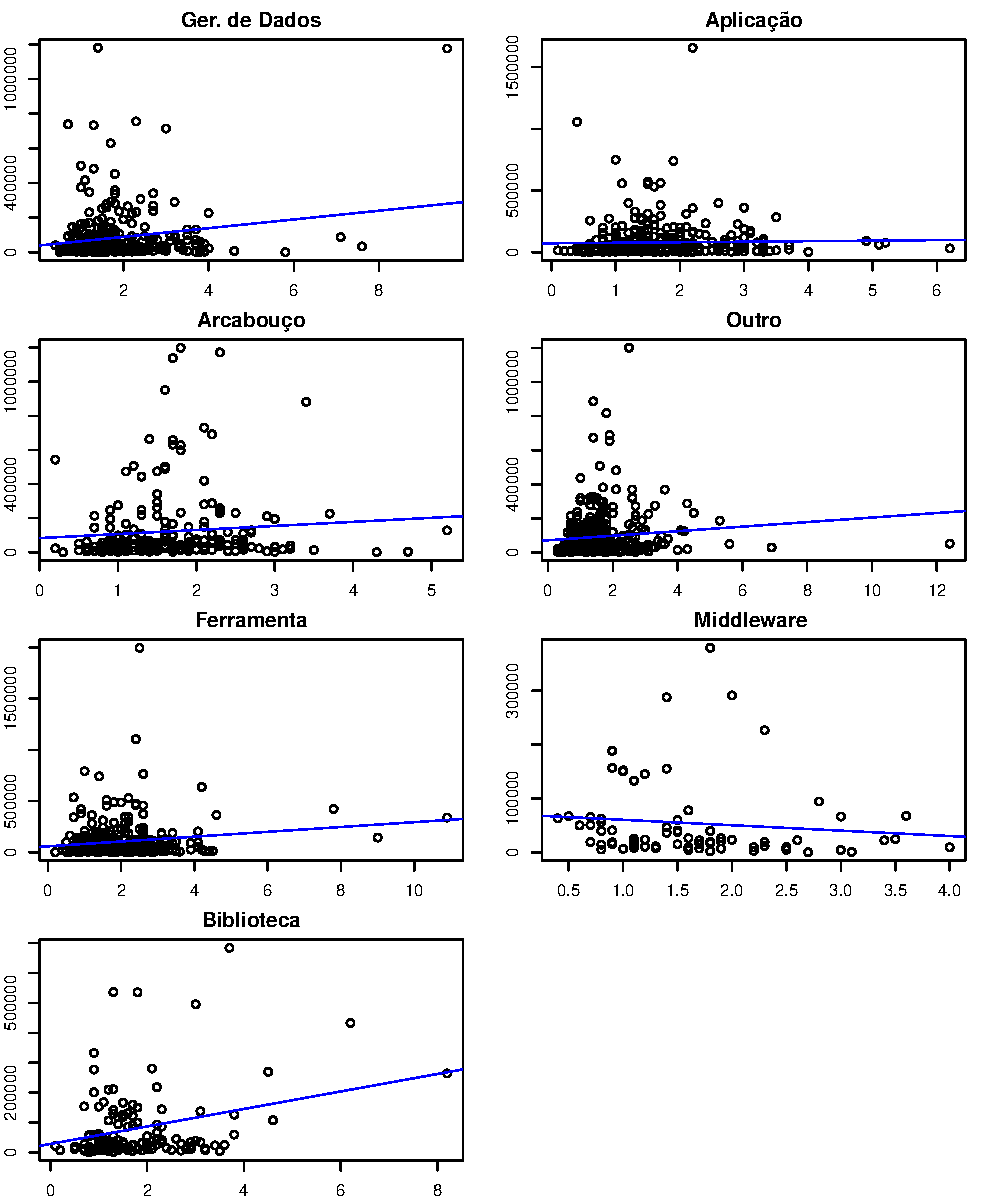
\includegraphics[trim={0cm 0cm 0cm 0cm},clip]{capitulo_estudo_caso/analise_exploratoria/correlacao_divida_nloc.pdf}} 
  \caption{Correlação entre a dívida técnica e a quantidade de linhas de código.}
  \label{fig:correlacao_divida_linhas_codigo} 
\end{figure}

 \begin{figure}[H]
  \centering
  \frame{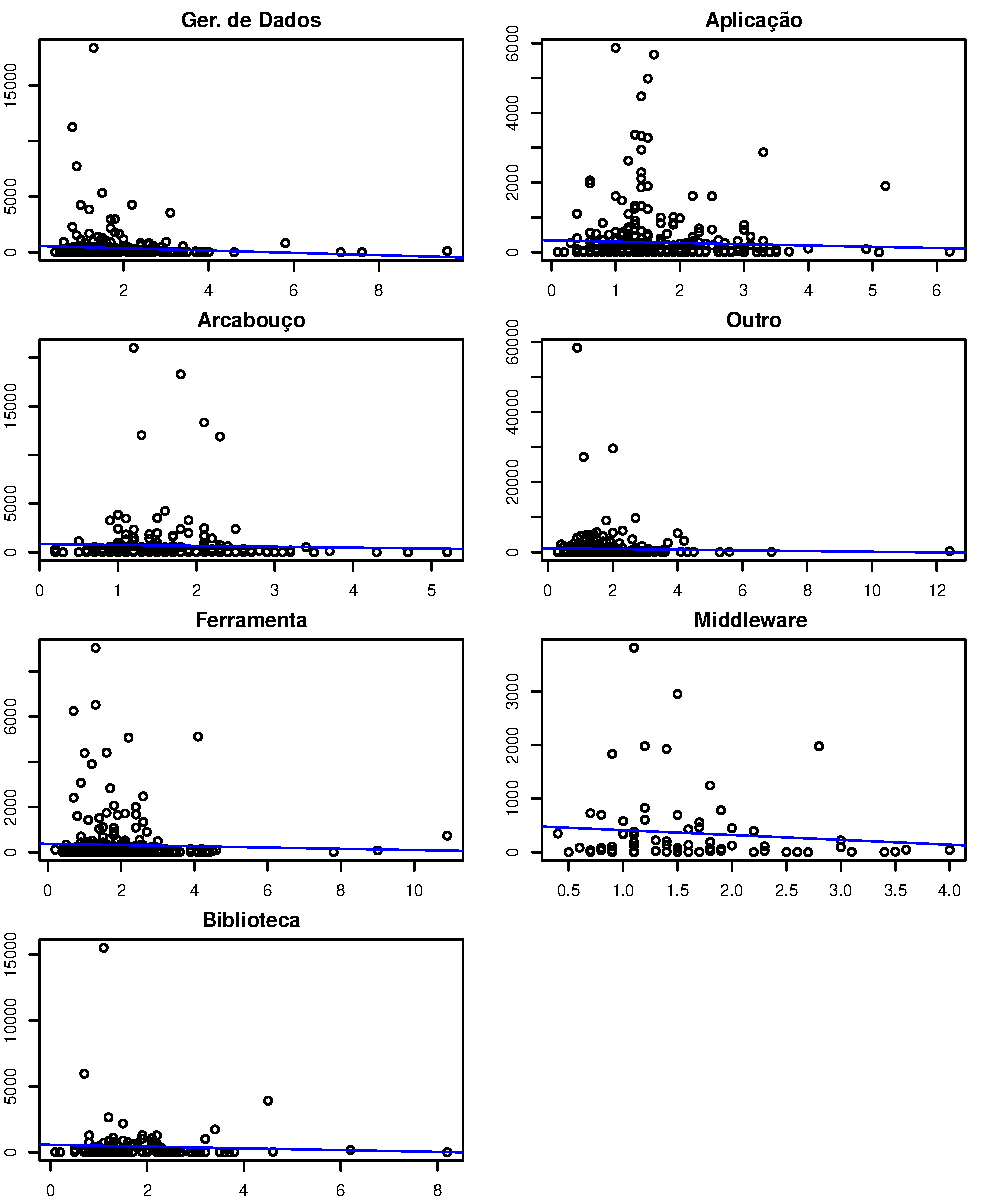
\includegraphics[trim={0cm 0cm 0cm 0cm},clip]{capitulo_estudo_caso/analise_exploratoria/correlacao_divida_watchers.pdf}} 
  \caption{Correlação entre a dívida técnica e a quantidade de \textit{watchers}.}
  \label{fig:correlacao_divida_watchers} 
\end{figure}


 \begin{figure}[H]
  \centering
  \frame{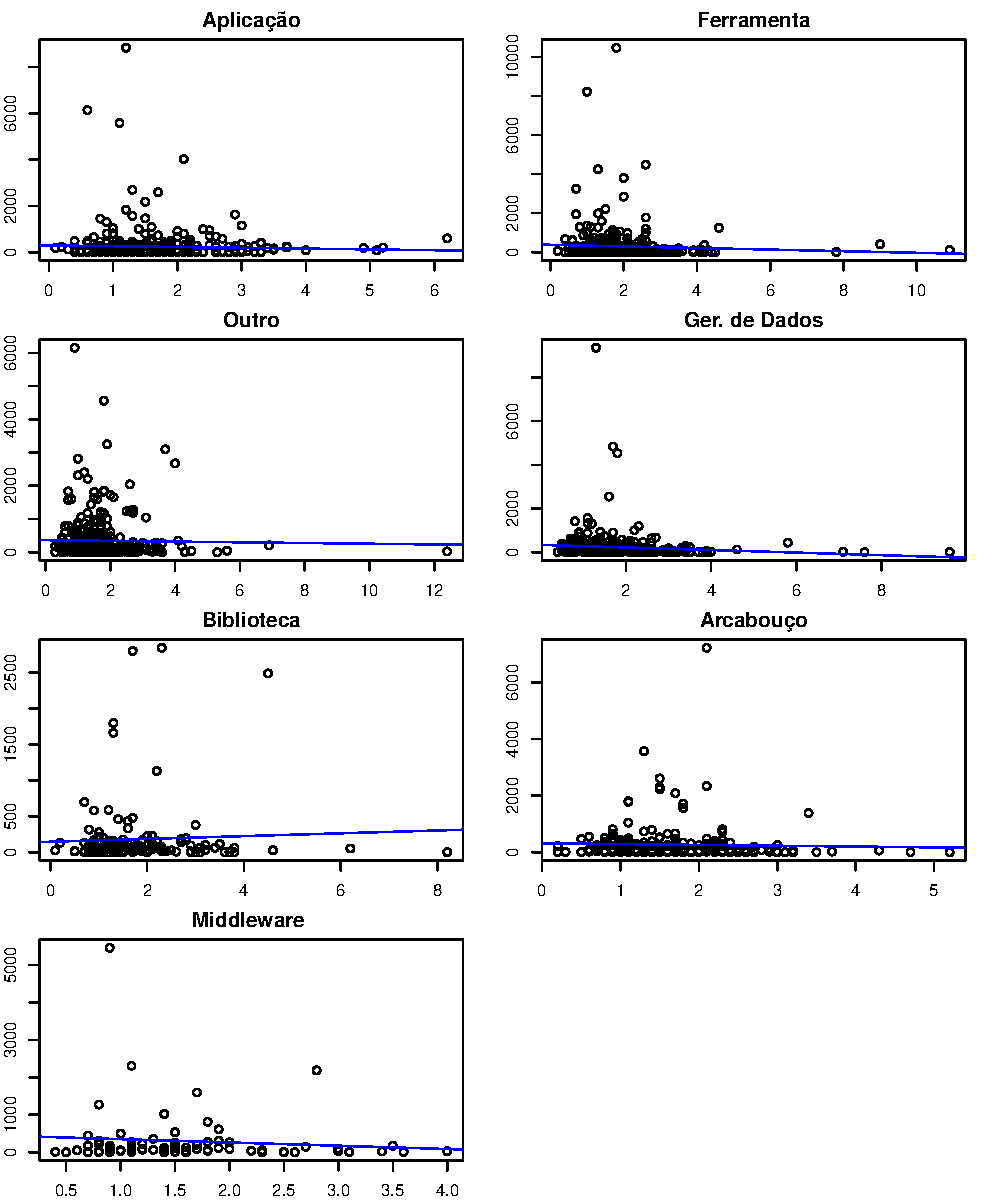
\includegraphics[trim={0cm 0cm 0cm 0cm},clip]{capitulo_estudo_caso/analise_exploratoria/correlacao_divida_pull_request.pdf}} 
  \caption{Correlação entre a dívida técnica e a quantidade de \textit{Pull requests}.}
  \label{fig:correlacao_divida_pull_request} 
\end{figure}


\subsection{Colaboração}

IN PROGRESS

\subsection{Produtividade}

IN PROGRESS

\subsection{Estimação dos juros}

IN PROGRESS







